\documentclass[a4j]{ujarticle}
\usepackage[dvipdfmx]{graphicx}
\usepackage{url}
\usepackage{bbding}
\usepackage{lscape}
\usepackage[subrefformat=parens]{subcaption}
\usepackage{bm}
\usepackage{amsmath}

\title{ミーティング資料}
\author{安達智哉\\to-adachi@ist.osaka-u.ac.jp}
\date{2019年6月19日}

\begin{document}
\maketitle


\section{MMEにおけるメモリ負荷の算出}
\label{seq:mme_memory}
\subsection{UEの状態遷移に伴うメモリ負荷}
文献\cite{3gpp.23.720}に示されているコネクション確立に伴うシグナリング図を図\ref{Legacy_connection_setup}に示す。
UEがIdle状態からConnected状態へ遷移する際に各ノードのメモリが保持する情報についてOAIのソースコード(OpenairinterfaceCN-develop)を元に調査を行っている。
具体的には、各シグナリングを処理する際に各ノードがメモリに格納する情報をリストアップし、それらの情報量を足し合わせることによりメモリ負荷を推定する。
今回は、MMEが関与している以下のシグナリングを処理する際にMMEが保持する情報を調査した。
\begin{itemize}
  \item S1-AP Initial UE msg
  \item S1-AP Initial Ctxt Setup Request
  \item S1-AP Initital Ctxt Setup Compl
  \item Modify Bearer Request
  \item Modify Bearer Response
  \item S1-AP UE Ctxt Release Req
  \item Release Access Bearers Req
  \item Release Access Bearers Resp
  \item S1-AP UE Ctxt Release Cmd
  \item S1-AP UE Ctxt Release Compl
\end{itemize}
\begin{figure}[htbp]
  \centering
  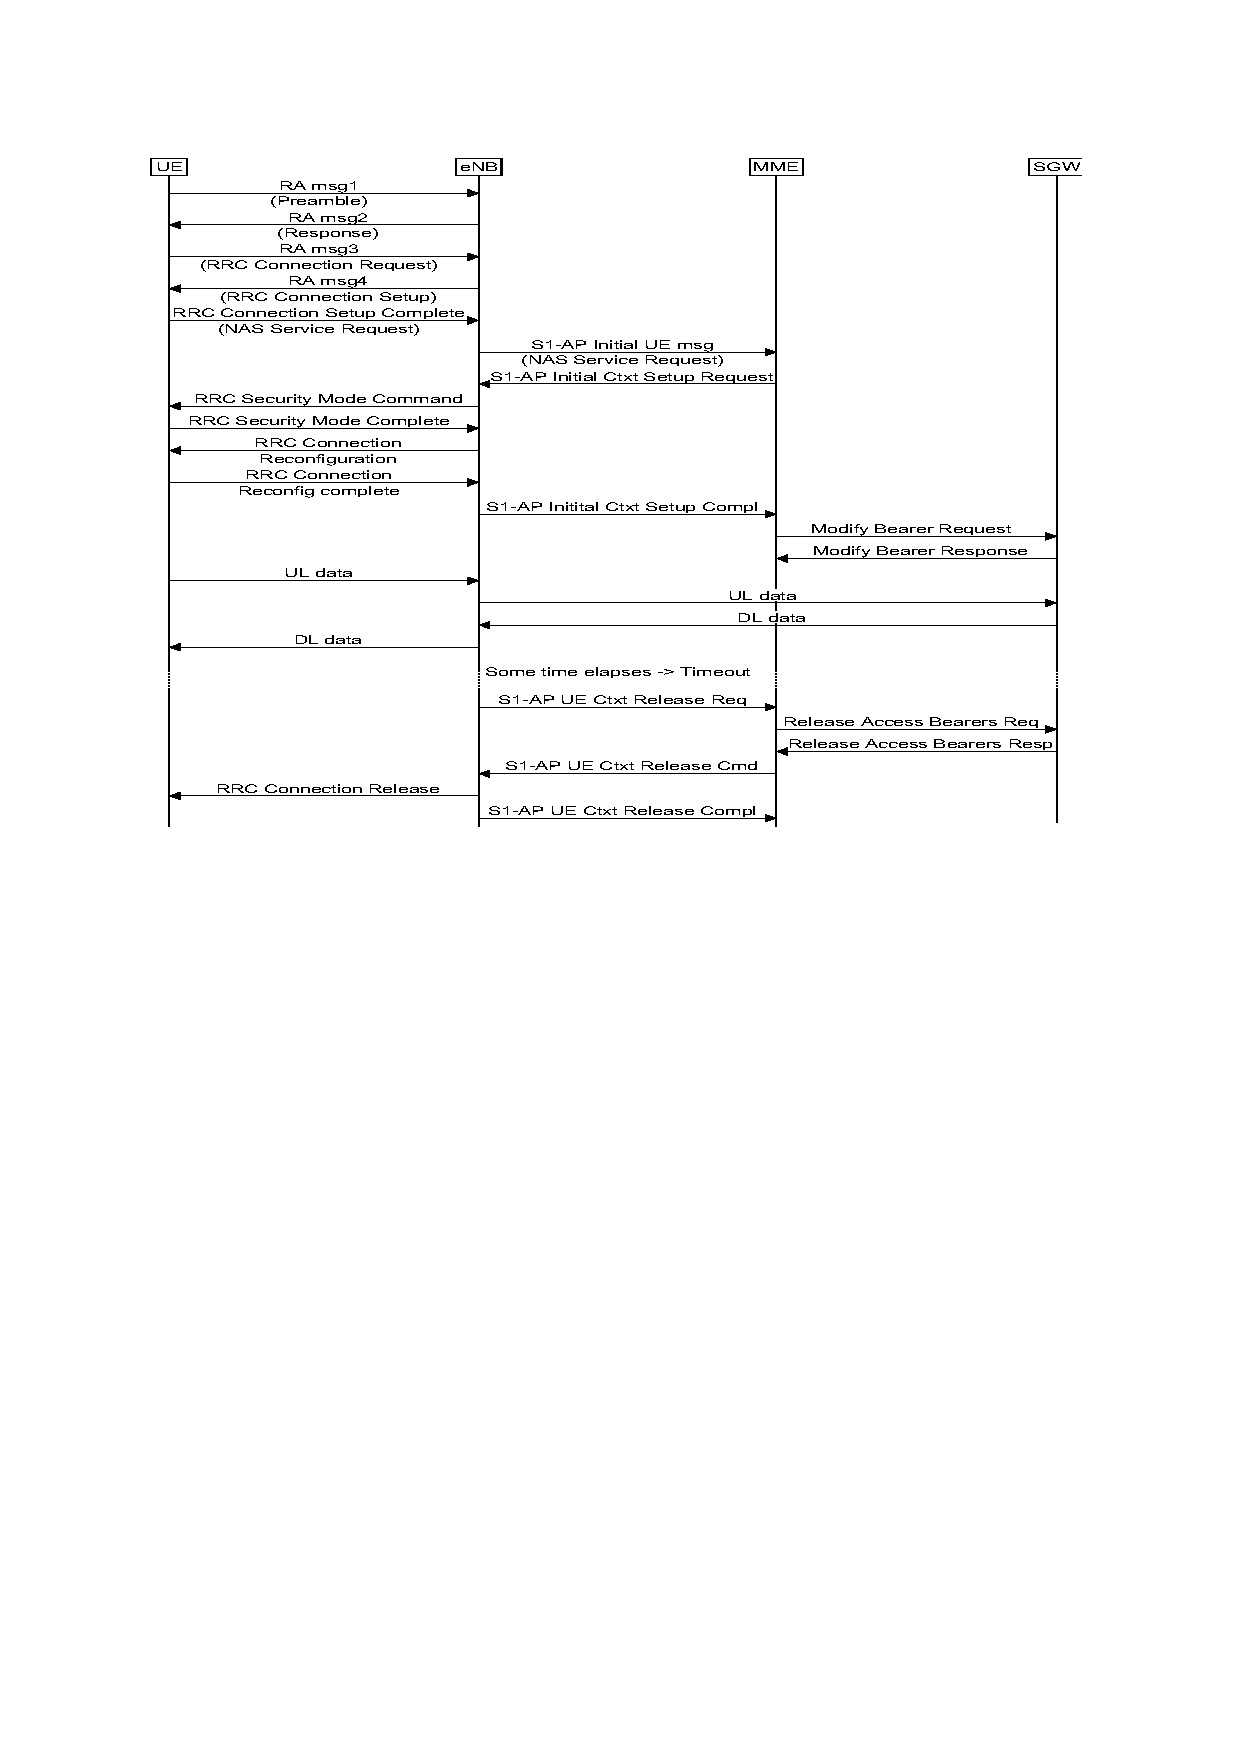
\includegraphics[width=0.9\hsize]{Legacy_connection_setup.pdf}
  \caption{Legacy connection setup}
  \label{Legacy_connection_setup}
\end{figure}


\clearpage
MMEが各シグナリングを受信、送信する際に保持する情報を以下の表\ref{table:oai_source_memory}に示す。

S1-AP Initial UE msgを受信した際は、約2KBの分の構造体を生成しており、この構造体にUEのコンテキストやベアラ情報を格納している。
S1-AP Initital Ctxt Setup Complの受信とModify Bearer Requestの送信処理では、メモリに情報を追加する処理は行っていない。
Modify Bearer Responseを受信した際は、MMEの持つUEのステートに関する情報の更新を行っている。
しかし、メモリに保持する情報量に変化はない。


S1-AP UE Ctxt Release Reqを受信した際は、MMEが保持しているUEのステートをConnectedからIdleへ変更する処理や次のシグナリングであるRelease Access Bearers Reqの準備等を行っているが、メモリに保持する情報の追加や削除は行われていない。
Release Access Bearers Reqの送信の処理処理ではメモリ操作はない。
Release Access Bearers Respを受信してからS1-AP UE Ctxt Release Cmdを送信するまでの処理で、MMEの管理するベアラ情報の更新を行う。
S1-AP UE Ctxt Release Complを受信した際に UEのコンテキストを削除している。


\begin{table}[htbp]
  \centering
  \caption{シグナリングメッセージを処理する際にMMEが保持する情報}
  \label{table:oai_source_memory}
  \begin{tabular}{l|l|c}
    \hline
    シグナリング  & 情報名 & 情報量(bit)  \\ \hline \hline
    S1-AP Initial UE msg & \verb|ue_description_s| & 408 \\
    & \verb|ue_context_s| & 17470\\\hline
    S1-AP Initital Ctxt Setup Compl & - & 0 \\\hline
    Modify Bearer Request & - & 0 \\\hline
    Modify Bearer Response & - & 0 \\\hline
    S1-AP UE Ctxt Release Req & - & 0 \\\hline
    Release Access Bearers Req & - & 0 \\\hline
    Release Access Bearers Resp & - & 0 \\\hline
    S1-AP UE Ctxt Release Compl & \verb|ue_context_s| & -17470 \\\hline

  \end{tabular}
\end{table}

S1-AP Initial UE msgを処理する際にMMEは、\verb|ue_description_s|および\verb|ue_context_s|という名前の構造体を保持することが表\ref{table:oai_source_memory}より分かる。この構造体の中身を以下の表\ref{table:oai_source_memory_ue_description_s}、表\ref{table:oai_source_ue_context_s}に示す。
\begin{table}[htbp]
  \centering
  \caption{ue\_description\_sのメンバ}
  \label{table:oai_source_memory_ue_description_s}
  \begin{tabular}{l|l}
    \hline
    メンバ & 情報量(bit) \\ \hline \hline
    \verb|enb_description_s| & 32\\
    \verb|s1_ue_state_s| & 160\\
    \verb|enb_ue_s1ap_id_t|  & 24\\
    \verb|mme_ue_s1ap_id_t| & 32\\
    \verb|sctp_stream_id_t (s ctp_stream_recv)| & 16\\
    \verb|sctp_stream_id_t (s ctp_stream_send)| & 16\\
    \verb|s11_sgw_teid| & 32\\
    \verb|outcome_response_timer_id| & 32\\
    \verb|s1ap_ue_context_rel_timer| & 64\\\hline
    合計  & 408\\\hline
  \end{tabular}
\end{table}

\begin{table}[htbp]
  \centering
  \caption{ue\_context\_sのメンバ}
  \label{table:oai_source_ue_context_s}
  \begin{tabular}{l|l}
    \hline
    メンバ & 情報量(bit) \\ \hline \hline
    \verb|imsi| & 64\\
    \verb|imsi_auth| & 1\\
    \verb|enb_s1ap_id_key_t| & 64\\
    \verb|enb_ue_s1ap_id_t| & 24\\
    \verb|mme_ue_s1ap_id_t | & 32\\
    \verb|sctp_assoc_id_t | & 32\\
    \verb|ue_context_rel_cause| & 224\\ %441
    \verb|subscription_known| & 1\\
    \verb|msisdn[MSISDN_LENGTH+1]| & 128\\
    \verb|msisdn_length| & 8\\
    \verb|mm_state| & 64\\
    \verb|ecm_state| & 64\\
    \verb|is_guti_set| & 8\\
    \verb|guti| & 80\\ %353
    \verb|me_identity| & 240\\
    \verb|e_utran_cgi| & 56\\
    \verb|cell_age| & 64\\
    \verb|access_mode| &128 \\
    \verb|apn_profile| &356 \\
    \verb|access_restriction_data| & 32\\%876
    \verb|sub_status| & 96\\
    \verb|subscribed_ambr| & 128\\
    \verb|used_ambr| & 128\\
    \verb|rau_tau_timer| & 32\\
    \verb|*ue_radio_capabilities| & 8\\
    \verb|ue_radio_cap_length| & 32\\
    \verb|mme_s11_teid| & 32\\
    \verb|sgw_s11_teid| & 32\\
    \verb|paa| & 328\\%816
    \verb|pending_pdn_connectivity_req_imsi[16]| & 128\\
    \verb|pending_pdn_connectivity_req_imsi_length| & 8\\
    \verb|pending_pdn_connectivity_req_apn| & 72\\
    \verb|pending_pdn_connectivity_req_pdn_addr| & 72\\
    \verb|pending_pdn_connectivity_req_pti| & 32\\
    \verb|pending_pdn_connectivity_req_ue_id| & 32\\
    \verb|pending_pdn_connectivity_req_qos| & 160\\
    \verb|pending_pdn_connectivity_req_pco| & 784\\
    \verb|pending_pdn_connectivity_req_request_type| & 32\\
    \verb|default_bearer_id| & 8\\
    \verb|eps_bearers[BEARERS_PER_UE]| & 13464\\
    \verb|mobile_reachability_timer| & 64\\
    \verb|implicit_detach_timer| & 64\\
    \verb|initial_context_setup_rsp_timer| & 64\\\hline%14984
    合計  & 17470\\\hline
  \end{tabular}
\end{table}

\clearpage
今回の調査の結果と文献\cite{ANovelStateModelfor5GRadioAccessNetworks}で示されている、RRC Connected Inactive 状態からConnected状態へ遷移する際のシグナリング図(図\ref{Signaling_for_the_RRC_CONNECTED_INACTIVE_to_RRC_CONNECTED_transition_for_the_novel_state_model})を参考にすることにより、各状態にあるUEがMMEに与えるメモリ負荷を推定することができた。
結果を表\ref{table:OAI_mme_memory}に示す。

図\ref{Signaling_for_the_RRC_CONNECTED_INACTIVE_to_RRC_CONNECTED_transition_for_the_novel_state_model}を見ると、RRC Connected Inactive 状態からConnected状態へ遷移する際にはUE-RAN間のシグナリングが5回発生している一方、コアネットワーク側にはシグナリングは発生していないことがわかる。
よってRRC Connected Inactive 状態とConnected状態ではMMEの状態には変化がなく、メモリ負荷も同じであると言える。

\begin{figure}[htbp]
  \centering
  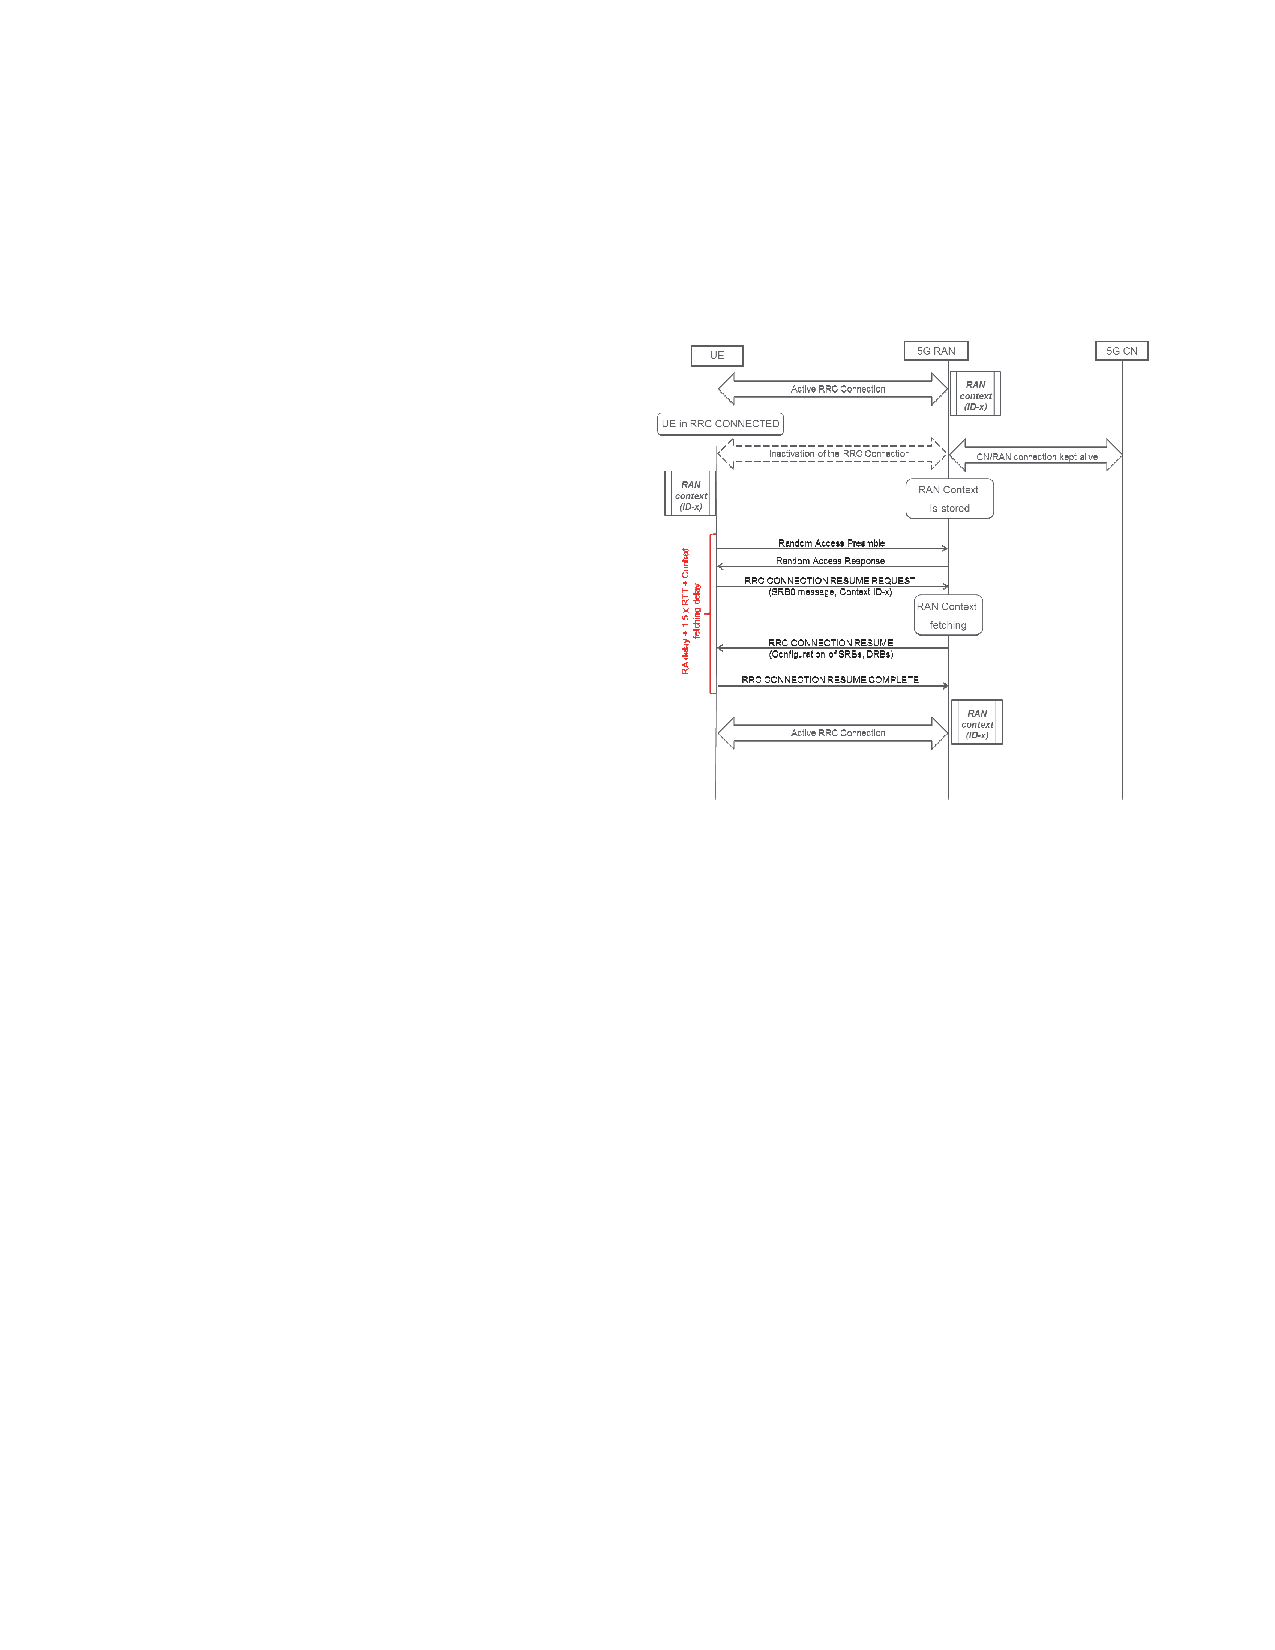
\includegraphics[width=0.9\hsize]{Signaling_for_the_RRC_CONNECTED_INACTIVE_to_RRC_CONNECTED_transition_for_the_novel_state_model.pdf}
  \caption{Signaling for the RRC CONNECTED INACTIVE to RRC CONNECTED transition for the novel state model}
  \label{Signaling_for_the_RRC_CONNECTED_INACTIVE_to_RRC_CONNECTED_transition_for_the_novel_state_model}
\end{figure}

\begin{table}[htbp]
  \centering
  \caption{MMEが保持する情報}
  \label{table:OAI_mme_memory}
  \begin{tabular}{l|l|c}
    \hline
    UEのステート  & 情報名 & 情報量(bit)  \\ \hline \hline
    Connected & \verb|ue_description_s| & 408 \\
    & \verb|ue_context_s| & 17470\\\hline
    Connected Inactive & \verb|ue_description_s| & 408 \\
    & \verb|ue_context_s| & 17470\\\hline
    Idle & \verb|ue_description_s| & 408 \\
  \end{tabular}
\end{table}

\clearpage


\subsection{eNodeBが追加された時のメモリ負荷}
新規のeNodeBが接続した際には、\verb|enb_description_s|という構造体が生成され、この情報をMMEが保持する。
この構造体の中身を表\ref{table:oai_source_enb_description_s}に示す。
この構造体のサイズは225 bytesであることが分かった。
\begin{table}[htbp]
  \centering
  \caption{enb\_description\_sのメンバ}
  \label{table:oai_source_enb_description_s}
  \begin{tabular}{l|l}
    \hline
    メンバ & 情報量(bit) \\ \hline \hline
    \verb|s1_state| & 128\\
    \verb|enb_name[150]| & 1200\\
    \verb|enb_id| & 32\\
    \verb|default_paging_drx| & 8\\
    \verb|nb_ue_associated| & 32\\ %1400
    \verb|ue_coll| & 320\\
    \verb|sctp_assoc_id| & 32\\
    \verb|next_sctp_stream| & 16\\
    \verb|instreams| & 16\\
    \verb|outstreams| & 16\\ \hline %400
    合計  & 1800\\\hline
  \end{tabular}
\end{table}

\section{シグナリング数の調査}
\label{seq:mme_signaling}
文献\cite{3gpp.23.720}および\cite{ANovelStateModelfor5GRadioAccessNetworks}を調査することにより、状態遷移に伴うシグナリングの発生数が明らかになった。
図\ref{state_id}に示す状態遷移図と共に、状態遷移に伴って発生するシグナリングに関する情報を、表\ref{table:signalings_all}に示す。

\begin{figure}[htbp]
  \centering
  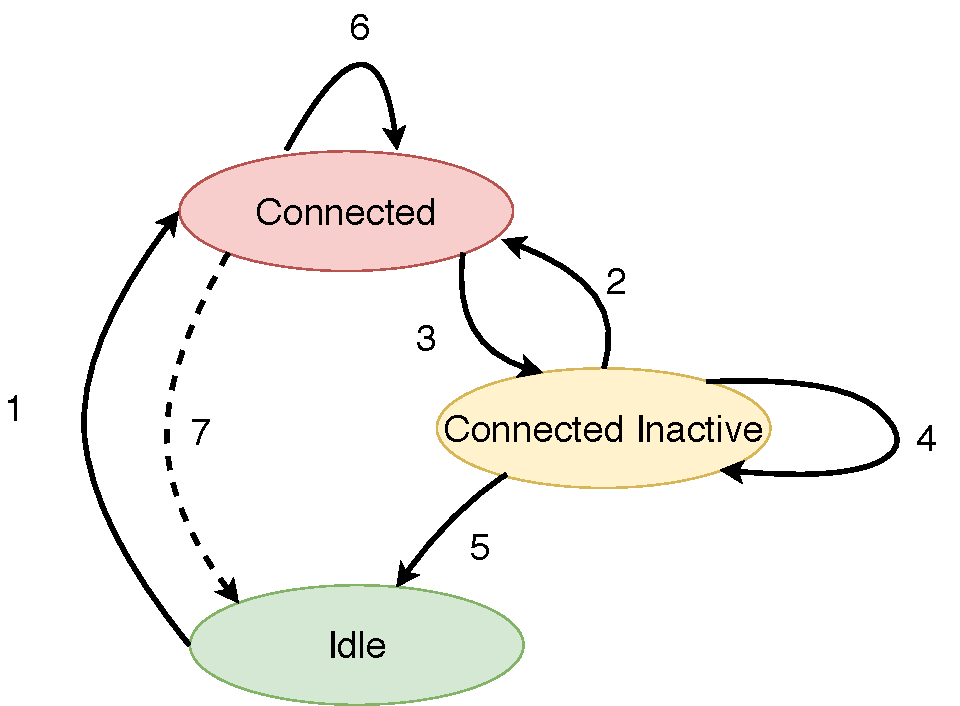
\includegraphics[width=0.9\hsize]{state_id.pdf}
  \caption{state transition}
  \label{state_id}
\end{figure}

\begin{table}[htbp]
  \centering
  \caption{Signaling Load}
  \label{table:signalings_all}
  \begin{tabular}{c|cccc|l}
    \hline
    遷移ID  & \multicolumn{4}{|c|}{シグナリング処理数} & 遷移条件                          \\
            & UE      & RAN     & MME     & SGW      &                                   \\ \hline \hline
    1       & 9       & 12      & 5       & 2        & Packets transmission              \\
    2       & 5       & 5       & 0       & 0        & 2 or more packets transmission    \\
    3       & 1       & 1       & 0       & 0        & Connected timer expiration        \\
    4       & 4       & 4       & 0       & 0        & One packet transmission           \\
    5       & 0       & 3       & 5       & 2        & Connected Inactive timer expiration             \\
    6       & 0       & 0       & 0       & 0        & Packets transmission              \\
    7       & 1       & 4       & 5       & 2        & Connected timer expiration            \\ \hline
  \end{tabular}
\end{table}



\section{考察}
今回の調査結果から、UEがIdle状態とConnected状態およびConnected Inactive状態にあるときにMMEのメモリに与える負荷が明らかになった。
今回の結果では、UE 1台がIdle状態である時は、約408 bitのメモリ負荷が発生していると考えられる。
またConnected状態およびConnected Inactive状態である時は、約17,878 bitのメモリ負荷が発生していると考えられる。

また、eNodeBが新しく追加された時は、約1,800bit のメモリ負荷が発生することも分かった。

ここで以前調査した、上野さんの実験データに基づくMMEのメモリ負荷を図\ref{fig:mme_memory}に示す。
この図では、UE及びeNodeBを増加させつつUEのアタッチ処理を完了した際にどれほどのメモリ負荷がMMEに発生するかを示している。
図の結果では、UE1台のアタッチ処理のために約750 KBのメモリ負荷が発生している。

図\ref{fig:mme_memory}の結果と今回の調査結果は直接比較することはが、2桁ほどずれている点は留意すべきである。
上野さんに確認したところ、図\ref{fig:mme_memory}の結果はMMEを起動しているシステム全体のメモリ消費を見ているということであるため、OAI以外のレイヤーの通信プロトコルの処理負荷も含まれていることが分かった。
図\ref{fig:mme_memory}の結果と今回の調査結果の間で大きなずれがある理由は、他の通信プロトコルの負荷の影響である可能性が高い。
\begin{figure}[htbp]
  \centering
  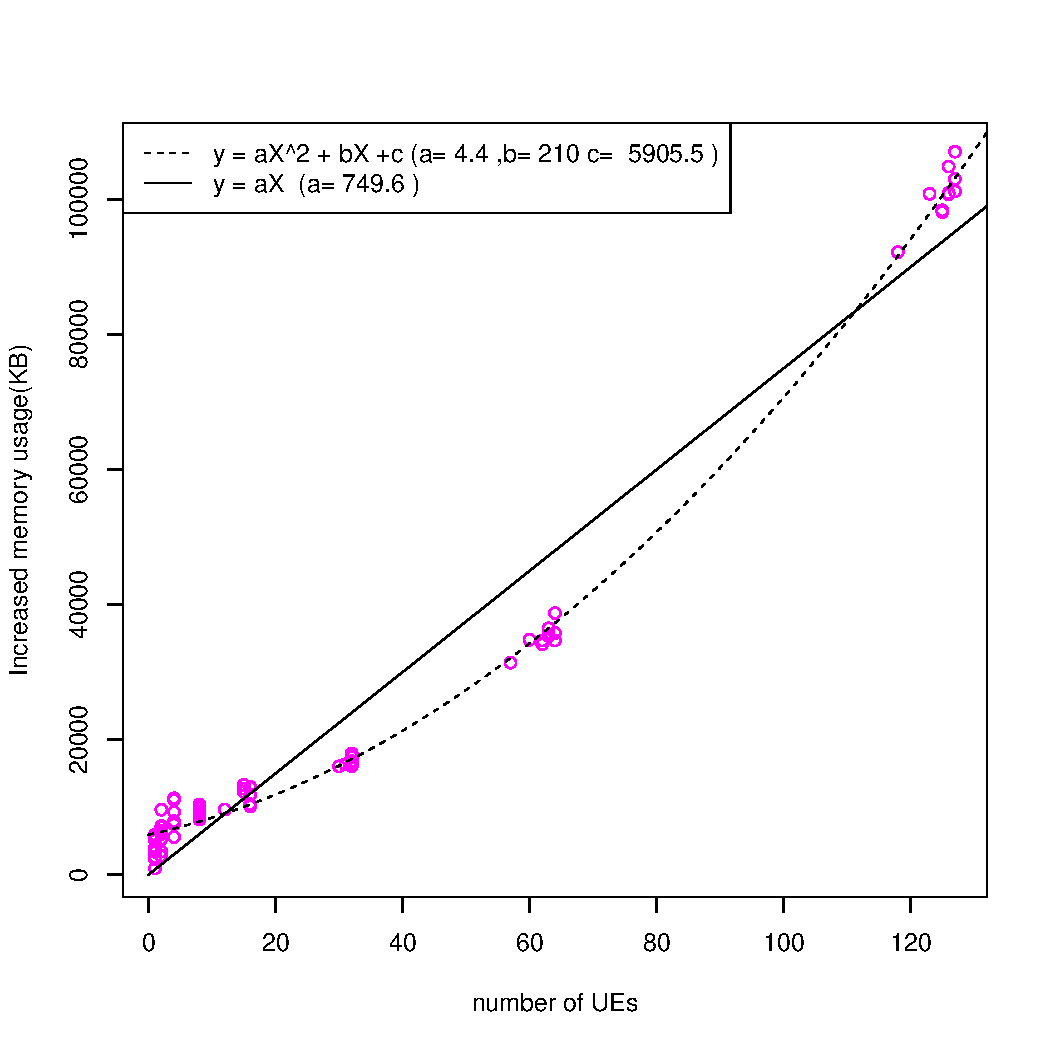
\includegraphics[width=0.9\hsize]{mme_memory.pdf}
  \caption{UE、eNodeBの増加とアタッチ処理の完了によって増加したメモリ負荷(MME)}
  \label{fig:mme_memory}
\end{figure}

\clearpage
\section{MMEの負荷の試算方法}
\label{seq:estimate}
MMEの負荷に合わせて、UEの状態を制御することにより、どの程度メモリおよびCPUに与える負荷のバランスを変化させることが可能であるかを試算する。
UEの状態の制御は、UEが最後にデータを送信したあと、Idle状態に遷移するまでの時間 ($T^{\rm i}$) を設定することで実現する。
例えば、CPUが過負荷である場合は、$T^{\rm i}$を長く設定することにより、どの程度メモリの負荷が増加し、CPUの負荷が低下するかを試算する。
またその逆に、メモリが過負荷である場合は、$T^{\rm i}$を短く設定することにより、どの程度CPUの負荷が増加し、メモリの負荷が低下するかを調べる。

試算を行う上で決定するべきパラメータを以下に示す。
\begin{itemize}
  \item UEの通信周期: $D$
  \item 最後のデータ送信からConnected Inactive状態へ遷移するまでの時間: $T^{\rm ci}$
\end{itemize}
\subsection{CPU負荷の算出}
\label{sec:cpu}
ネットワーク全体におけるシグナリングの発生レートを求める。
$N_{\rm UE}$台のUEがネットワークに存在すると仮定した時のUEの集合$\bm{U}$を、$\bm{U} = \left\{ u_1,u_2,\ldots,u_{N_{\rm UE}} \right\}$と定義する。
あるUE $u_h$ $(u_h \in \bm{U})$が1秒あたりに発生させるシグナリングの数を$s_h$と定義する。
Connected Inactive状態では、小さいデータ量であれば、コントロールプレーンを使ってデータ送信を完了させることが可能である。
この場合、Connected状態への状態遷移は発生しない。状態遷移が発生しない送信が可能であるデータサイズの上限を$\alpha$とした時、UE $u_h$がデータ送信を行う際に、そのデータサイズが$\alpha$を超える割合を$d_h$ とする。
最後のデータ送信からConnected Inactive状態へ遷移するまでの時間を$T^{\rm ci}$、最後のデータ送信からIdle状態へ遷移するまでの時間を$T^{\rm i}$、$u_h$の通信周期を$T_h$とする。
また、状態遷移に伴うシグナリングの発生回数をそれぞれ表\ref{table:state}のように定義すると、$s_h$は以下の式(\ref{eq:attach_detach})で表せる。
ここで留意すべきは、$T_h$が$T^{\rm ci}$以下であるようなUEは、一度Connected状態に遷移すると、常時Connected状態を維持し、状態遷移によるシグナリングが発生しないため、$s_h$は0と定義したことである。
また、私の研究では$T^{\rm i}$を制御するのであるが、この値が$T^{\rm ci}$以下になるような設定はしないことを前提にしている。そのため以下の式でも$T^{\rm i} >= T^{\rm ci}$が常に成り立つものとしている。
\begin{table}[h]
 \caption{state signaling}
 \label{table:state}
 \centering
  \begin{tabular}{ccc}
   \hline
   Source & Destination & The number of signaling occurrences \\
   \hline \hline
   Connected & Connected & $n_{\rm MME}^{\rm c \to \rm c}$ \\
   Connected Inactive & Connected Inactive & $n_{\rm MME}^{\rm ci \to \rm ci}$ \\
   Connected & Connected Inactive & $n_{\rm MME}^{\rm c \to \rm ci}$ \\
   Connected Inactive & Connected & $n_{\rm MME}^{\rm ci \to \rm c}$ \\
   Connected Inactive & Idle & $n_{\rm MME}^{\rm ci \to \rm i}$ \\
   Idle & Connected  & $n_{\rm MME}^{\rm i \to \rm c}$ \\
   \hline
  \end{tabular}
\end{table}


\begin{equation}
  s_h  =
  \begin{cases}
		\frac{1}{T_h} \cdot n_{\rm MME}^{\rm c \to \rm c} & \text{if $T_h \le T^{\rm ci}$} \\
    \frac{1}{T_h} \cdot (n_{\rm MME}^{\rm ci \to \rm c} + n_{\rm MME}^{\rm c \to \rm ci}) \cdot d_h  + \frac{1}{T_h} \cdot n_{\rm MME}^{\rm ci \to \rm ci} \cdot (1 - d_h) & \text{if $T^{\rm ci} < T_h \le T^{\rm i}$} \\
    \frac{1}{T_h} \cdot (n_{\rm MME}^{\rm i \to \rm c} + n_{\rm MME}^{\rm c \to \rm ci} + n_{\rm MME}^{\rm ci \to \rm i}) & \text{otherwise}
  \end{cases}
  \label{eq:attach_detach}
\end{equation}

1秒毎にネットワーク全体で発生するシグナリングの合計を$S$と定義する。$S$は$s_h$を用いて以下の式(\ref{eq:all_signal})で表せる。
\begin{eqnarray}
  S & = & \sum_{h = 1}^{N_{\rm UE}} s_h \label{eq:all_signal}
\end{eqnarray}
この$S$より、CPUにかかる負荷を算出する。

\subsection{メモリ負荷の算出}
\label{sec:memory}
まず、UE $u_h$がConnected状態である時間割合を$p^{\rm c}_h$、Connected Inactive状態である時間割合を$p^{\rm ci}_h$、Idle状態である時間割合を$p^{\rm i}_h$と定義し、これらを求める。これらの値は、$T_h$および$T^{\rm i}$、$T^{\rm ci}$を用いて以下の式(\ref{eq:connected})、(\ref{eq:inactive})、(\ref{eq:idle})で表せる。
% ここでは、$s_h$が$T_i$以下であるようなUEは、常時接続状態となるため、$s_h$は1と定義した。
\begin{align}
	p^{\rm c}_h & =
	\begin{cases}
    1 \hphantom{100000000000000} & \text{if $T_h \le T^{\rm ci}$}\\
    \frac{T^{\rm ci}}{T_h} & \text{otherwise}
  \end{cases} \label{eq:connected}\\
	p^{\rm ci}_h & =
  \begin{cases}
    0 \hphantom{100000000000000} & \text{if $T_h \le T^{\rm ci}$}\\
		\frac{T_h - T^{\rm ci}}{T_h} & \text{if $T^{\rm ci} < T_h \le T^{\rm i}$}\\
    \frac{T^{\rm i} - T^{\rm ci}}{T_h} & \text{otherwise}
  \end{cases} \label{eq:inactive}\\
	p^{\rm i}_h & =
  \begin{cases}
    0 \hphantom{100000000000000} & \text{if $T_h \le T^{\rm ci}$}\\
		0 & \text{if $T^{\rm ci} < T_h \le T^{\rm i}$}\\
    \frac{T_h - T^{\rm i}}{T_h} & \text{otherwise}
  \end{cases}\label{eq:idle}
\end{align}

\begin{align}
	p^{\rm c}_h & =
	\begin{cases}
    1 \hphantom{100000000000000} & \text{if $T_h \le T^{\rm ci}$}\\
    \frac{T^{\rm ci}}{T_h} \cdot d_h + \frac{0}{T_h} \cdot (1 - d_h)& \text{if $T^{\rm ci} < T_h \le T^{\rm i}$}\\
    \frac{T^{\rm ci}}{T_h} & \text{otherwise}
  \end{cases} \label{eq:connected}\\
	p^{\rm ci}_h & =
  \begin{cases}
    0 \hphantom{100000000000000} & \text{if $T_h \le T^{\rm ci}$}\\
		\frac{T_h - T^{\rm ci}}{T_h} \cdot d_h + \frac{T_h}{T_h} \cdot (1 - d_h) & \text{if $T^{\rm ci} < T_h \le T^{\rm i}$}\\
    \frac{T^{\rm i} - T^{\rm ci}}{T_h} & \text{otherwise}
  \end{cases} \label{eq:inactive}\\
	p^{\rm i}_h & =
  \begin{cases}
    0 \hphantom{100000000000000} & \text{if $T_h \le T^{\rm ci}$}\\
		0 & \text{if $T^{\rm ci} < T_h \le T^{\rm i}$}\\
    \frac{T_h - T^{\rm i}}{T_h} & \text{otherwise}
  \end{cases}\label{eq:idle}
\end{align}

また、各状態におけるメモリ負荷をそれぞれ表\ref{table:state_memory}のように定義すると、UE $u_h$がMMEに与えるメモリ負荷の平均$b_h$は以下の式(\ref{eq:MME_memory})で表せる。

\begin{table}[h]
 \caption{各状態におけるUE1台当たりのMMEのメモリ負荷}
 \label{table:state_memory}
 \centering
  \begin{tabular}{cc}
   \hline
   state & load of MME memory \\
   \hline \hline
   Connected & $m^{\rm c}_{\rm MME}$ \\
   Connected Inactive & $m^{\rm ci}_{\rm MME}$ \\
   Idle & $m^{\rm i}_{\rm MME}$ \\
   \hline
  \end{tabular}
\end{table}

\begin{eqnarray}
  b_h & = & m^{\rm c}_{\rm MME} \cdot p^{\rm c}_h + m^{\rm ci}_{\rm MME} \cdot p^{\rm ci}_h + m^{\rm i}_{\rm MME} \cdot p^{\rm i}_h \label{eq:MME_memory}
\end{eqnarray}

MMEに対してネットワーク全体で発生する平均的なメモリ負荷の合計を$B$と定義する。$B$は$b_h$を用いて以下の式(\ref{eq:all_memory})で表せる。
\begin{eqnarray}
  B & = & \sum_{h = 1}^{N_{\rm UE}} b_h \label{eq:all_memory}
\end{eqnarray}


この$B$よりメモリ負荷を算出する。



\section{MME負荷の試算}
第\ref{seq:mme_memory}章で調査したメモリ負荷および、第\ref{seq:mme_signaling}章で調査したシグナリング負荷を参考にし、第\ref{seq:estimate}章で述べた数式を用いることで、MMEに発生する負荷を試算した。
今回、試算するにあたり、以下のように条件やパラメータを仮定した。
\begin{itemize}
  \item UEごとに通信周期は固定であり、途中で変化することはない。
  \item 最後の送信が終了したあと、Connected状態のUEがConnected Inactive状態へ遷移するまでの時間($T^{\rm ci}$)は全UEで共通かつ不変の値として$T^{\rm ci} = 10s$とした。
  \item UEの送信するデータサイズは十分大きいものとする。つまり、データ送信を行うタイミングで必ずConnected状態に遷移するものとする($d_h = 1$)。
  \item ネットワークに存在するUEの台数は600台とし、通信周期に対するUE台数の分布は以下の図\ref{UE_cycle}のように仮定する。つまり、通信周期に対してUEの台数は一様分布である。
  \item データ送信にかかる時間はUEの通信周期と比べて十分小さいものとし、送信が失敗することはないと仮定する。
\end{itemize}
\begin{figure}[htbp]
  \centering
  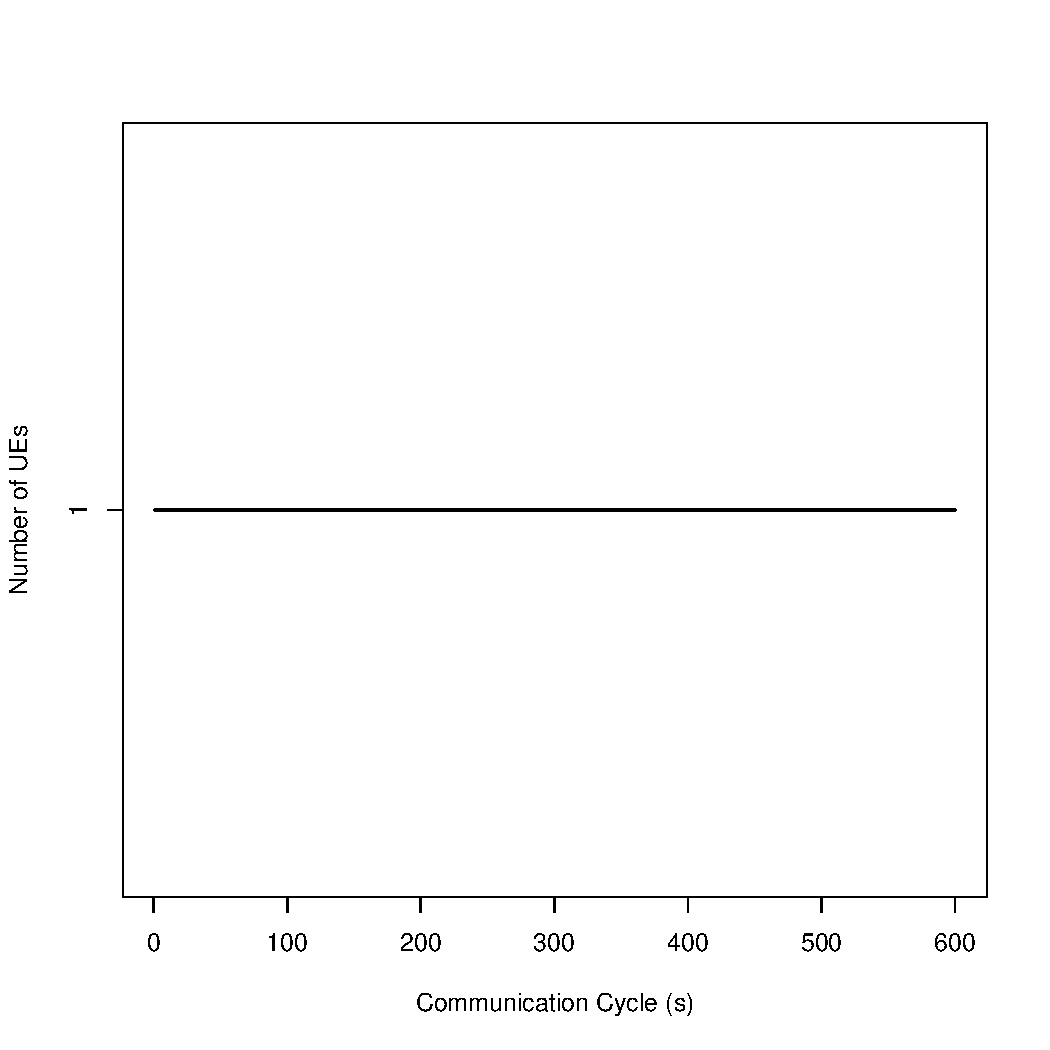
\includegraphics[width=0.9\hsize]{UE_cycle.pdf}
  \caption{通信周期に対するUE台数の分布}
  \label{UE_cycle}
\end{figure}


$T^{\rm i}$(最後のデータ送信からIdle状態へ遷移するまでの時間)を10sから600sの範囲で1sの精度で変化させた時に、MMEに対して発生する1sあたりのシグナリング数とMMEのメモリ負荷の変化を図\ref{signaling_and_memoryload_vs_idleTimer}に示す。

この図を見ると、$T^{\rm i}$の増加に対して、MMEのシグナリング負荷は単調減少であることが分かる。
これは、$T^{\rm i}$が増加することにより、Idle状態へ遷移するUEの台数が少なくなり、その分のシグナリングが削減されるからである。
また、$T^{\rm i}$の値が小さい時はMMEのシグナリング負荷の減少量が大きく、$T^{\rm i}$の値が大きい時はMMEのシグナリング負荷の減少量が小さいことも分かる。
これは、$T^{\rm i}$の値が小さい場合、$T^{\rm i}$の変化が影響を与えるのは通信周期が短いUE(シグナリング負荷への寄与が大きいUE)であり、$T^{\rm i}$の値が大きい場合、$T^{\rm i}$の変化が影響を与えるのは通信周期が長いUE(シグナリング負荷への寄与が小さいUE)であるからである。

また、$T^{\rm i}$の増加に対して、MMEのメモリ負荷は単調増加であることが分かる。
これは、$T^{\rm i}$が増加することにより、Idle状態へ遷移するまでの時間(Connected Inactive状態を維持する時間)が長くなるため、および、Idle状態へ遷移するUEの台数が少なくなるためである。
また、$T^{\rm i}$の値が小さい時はMMEのメモリ負荷の増加量が大きく、$T^{\rm i}$の値が大きい時はMMEのメモリ負荷の増加量が小さいことも分かる。
これは、$T^{\rm i}$の変化は$T^{\rm i}$よりも通信周期の長いUEの状態遷移に対してのみ変化を与えるためである。
つまり、$T^{\rm i}$の値が大きい場合は小さい場合と比べて、$T^{\rm i}$の変化が影響を与えるUE台数が減るため、メモリ負荷の変化量が小さくなっている。
\begin{figure}[htbp]
  \centering
  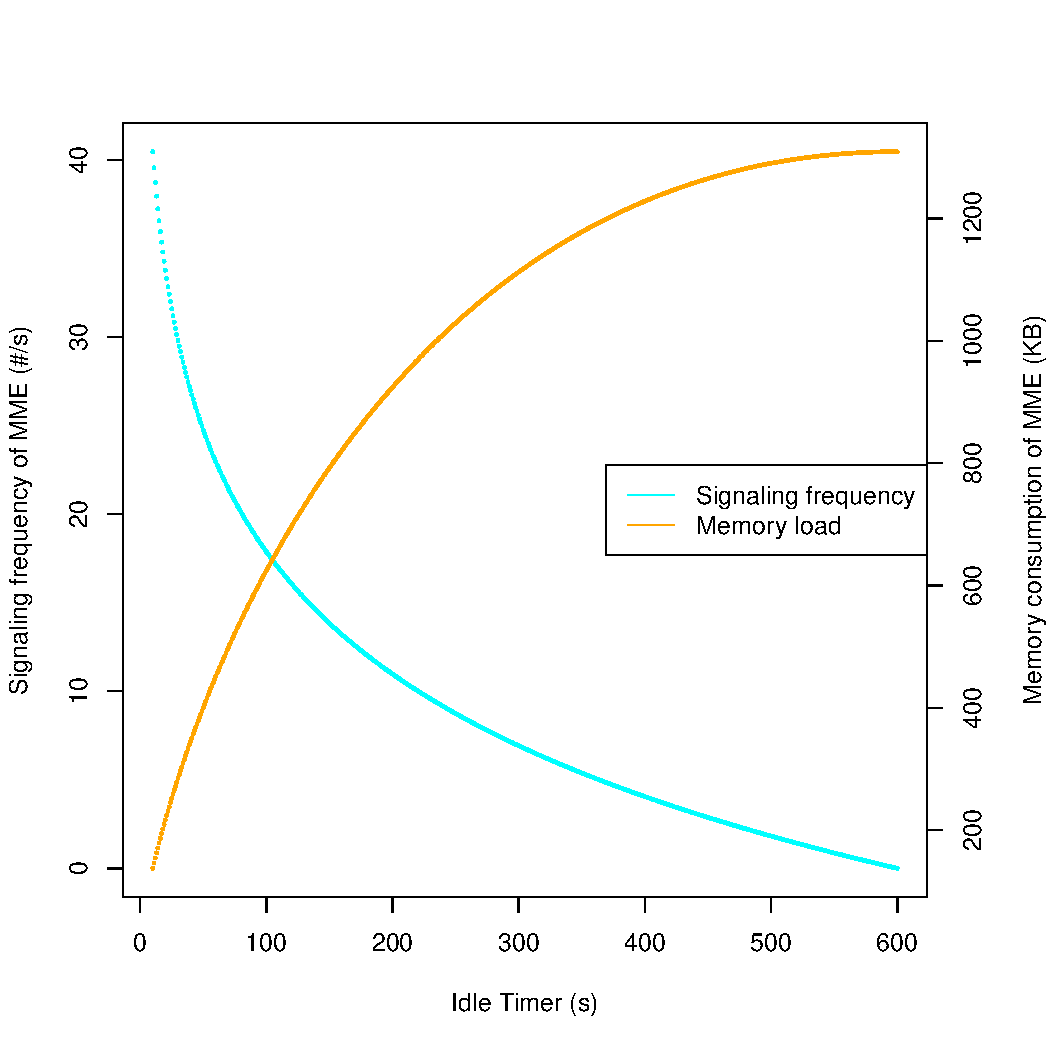
\includegraphics[width=0.9\hsize]{signaling_and_memoryload_vs_idleTimer.pdf}
  \caption{$T^{\rm i}$に対する、MMEに対して発生する1sあたりのシグナリング数とメモリ負荷}
  \label{signaling_and_memoryload_vs_idleTimer}
\end{figure}

MMEのシグナリング負荷とMMEのメモリ負荷の関係を示した図を図\ref{signaling_vs_memoryload}に示す。
\begin{figure}[htbp]
  \centering
  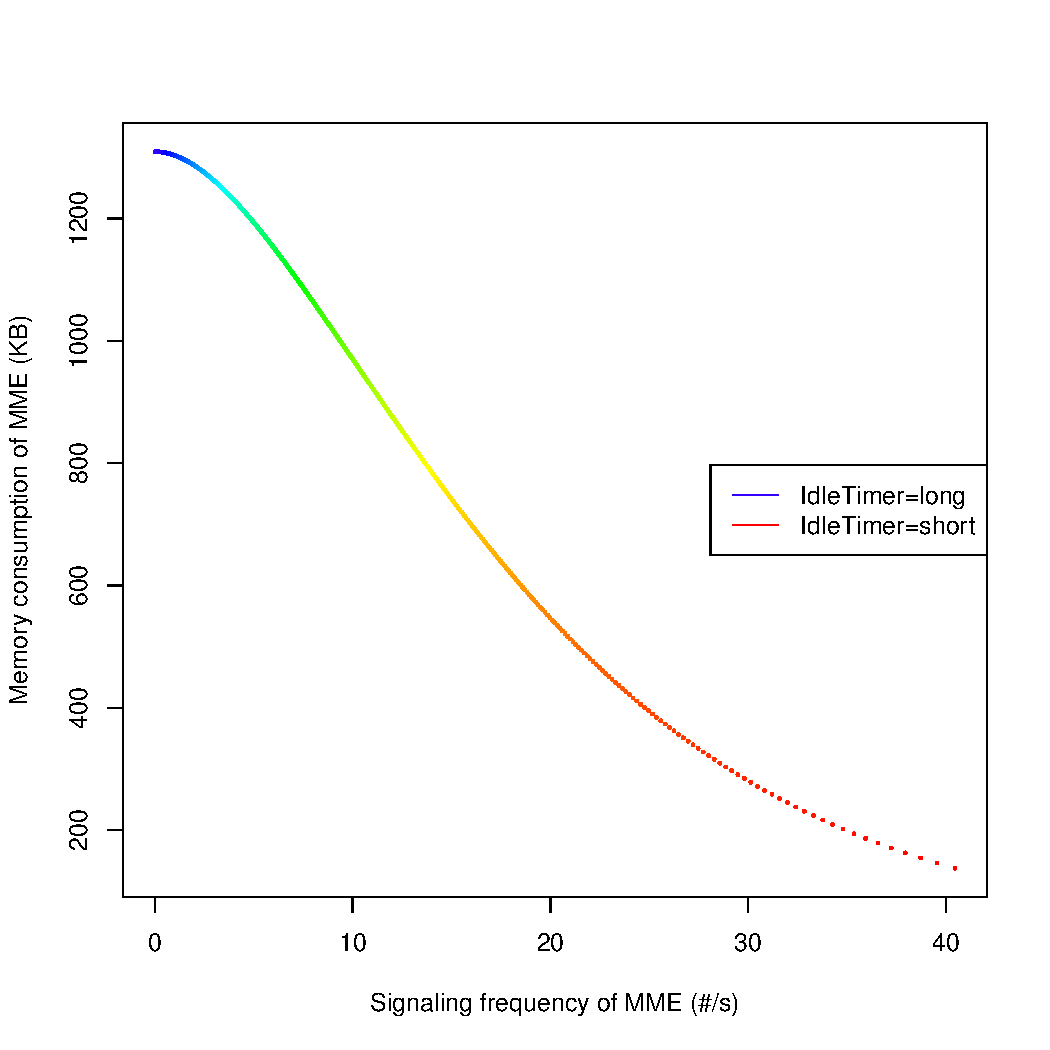
\includegraphics[width=0.9\hsize]{signaling_vs_memoryload.pdf}
  \caption{MMEに対して発生する1sあたりのシグナリング数に対するMMEのメモリ負荷}
  \label{signaling_vs_memoryload}
\end{figure}

\clearpage


\section{MMEが単位時間当たりに処理可能なシグナリングの最大数の推定}
図\ref{signaling_and_memoryload_vs_idleTimer}および図\ref{signaling_vs_memoryload}にIdleTimerとメモリ負荷およびシグナリング負荷の関係を示した。メモリ負荷に関してはMMEに搭載されているメモリのサイズや一般的なサーバに搭載されているメモリサイズなどと比較することにより、どの程度までの負荷が許容されるのかを議論することは容易である。

一方、シグナリング負荷に関しては、シグナリング負荷とCPU負荷との関係が自明でないため、負荷の許容範囲を明らかにすることは、一般的に容易ではない。そこで、今回は、上野さんの実験結果を参考にしつつ、どの程度までのシグナリング負荷が許容されるのかを推定した。

上野さんの論文\cite{多数のM2M/IoT端末からの集中アクセスを考慮したモバイルコアネットワークの実験評価}に示されている結果を図\ref{t_expect_ueno}および図\ref{Latency_node_ueno}に示す。
図\ref{t_expect_ueno}では、128台のUEが、特定の同期精度でアタッチ処理を開始した時に発生するレイテンシを示している。
同期精度は$T_{expect}$というパラメータで表現されている。
$T_{expect} = t$である時は、特定の時刻から$t$秒の範囲内でランダムに全UEがアタッチ処理を開始することを意味する。
この図を見ると$T_{expect}$の値が1.6以下になると、急激にレイテンシが増加していることがわかる。

また、図\ref{Latency_node_ueno}では、レイテンシの内訳を示している。
これを見ると、$T_{expect}$の値が1.6以下の時は、MMEのレイテンシが大幅に増加していることがわかる。
また、MMEのレイテンシが全体のレイテンシに対して大部分を占めていることもわかる。

以上の理由から、$T_{expect}$1.6以下の時に、128台のUEがアタッチ処理を開始した場合、MMEの処理にかかる遅延が大幅に増加することが分かる。
つまり、$T_{expect}$1.6以下の状況で、128台のUEがアタッチ処理を開始した時に発生する負荷は、MMEを過負荷状態にする。



\begin{figure}[htbp]
  \centering
  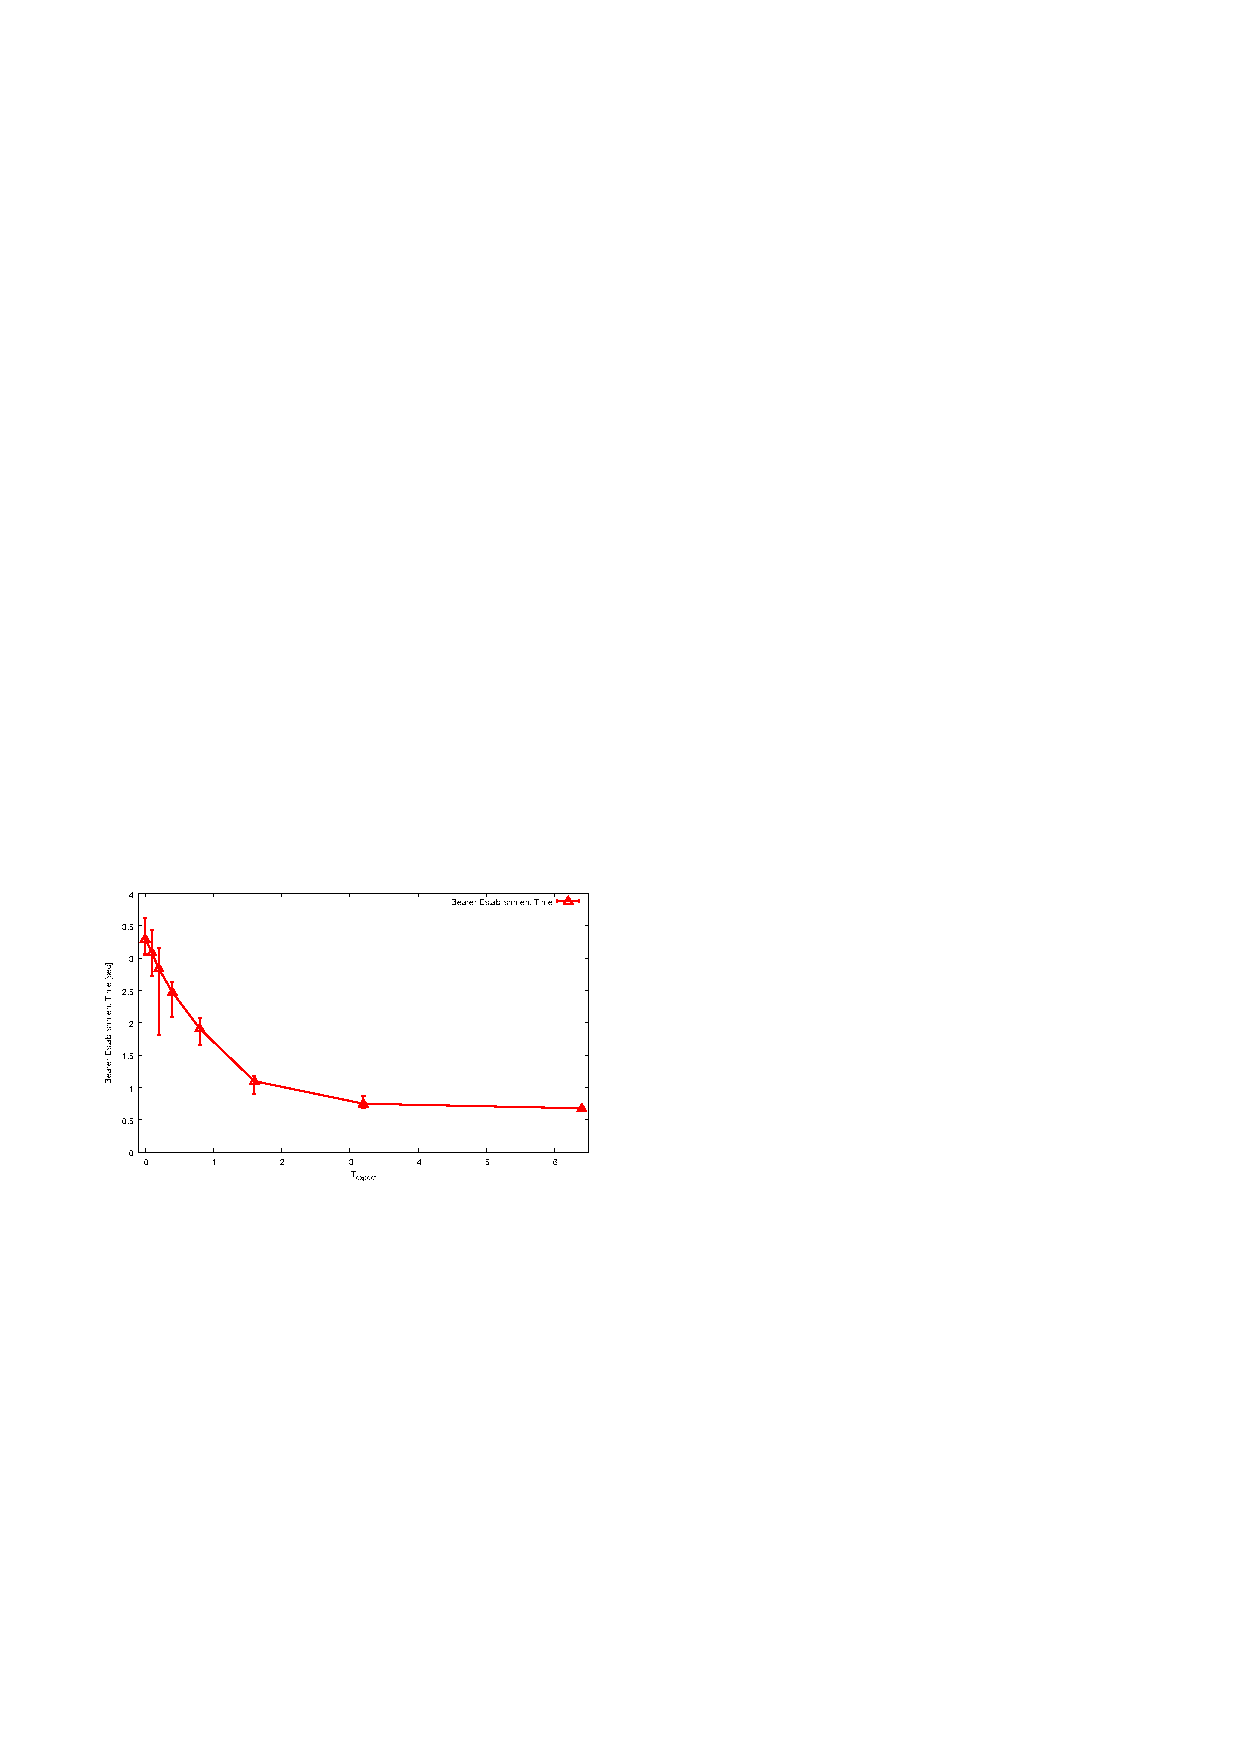
\includegraphics[width=0.6\hsize]{t_expect_ueno.pdf}
  \caption{Relationship between $T_{expect}$ and bearer establishmenttime}
  \label{t_expect_ueno}
\end{figure}

\begin{figure}[htbp]
  \centering
  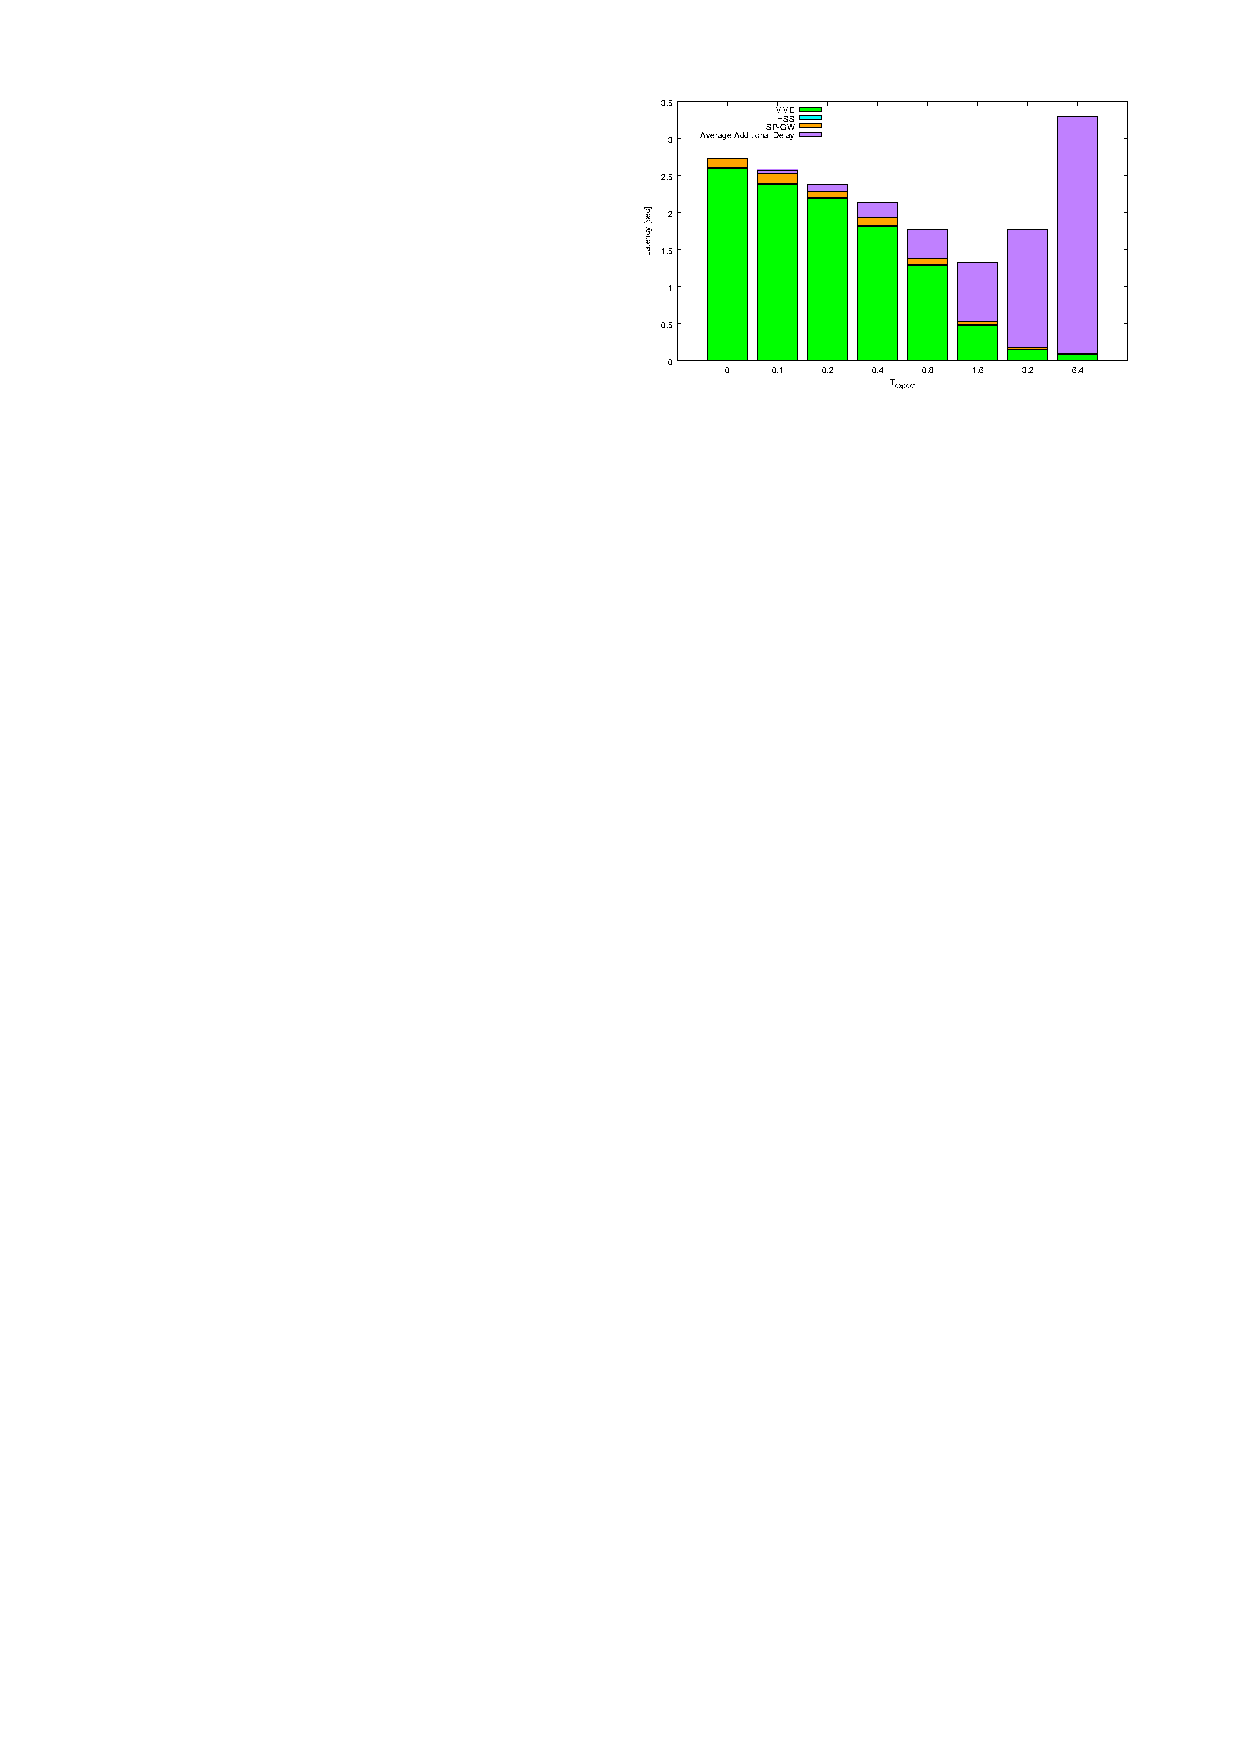
\includegraphics[width=0.6\hsize]{Latency_node_ueno.pdf}
  \caption{Relationship between $T_{expect}$ and signaling processing time on each EPC node}
  \label{Latency_node_ueno}
\end{figure}

% ここで留意するべきは、上野さんの実験から得られる情報は、ある特定の時刻において突発的にシグナリングが発生した場合のCPU負荷であるが、私が知りたい情報は、継続的にシグナリングが発生し続けるような場合のCPU負荷であり、両者は異なることである。そこで、以下に示すように、上野さんのデータを加工することにより、継続的にシグナリングが発生し続けるような場合のCPU負荷を推定した。
%
% 以下に上野さんの実験データとそれを加工したものを示す。これらのデータを用いて、何台のUEがアタッチ処理を実行するとMMEのCPUが過負荷になるのかを調査した。
%
% 図\ref{experiment_data_128_0001_mmeperf}に、128台のUEがアタッチ処理を実行した時の実験データを示す。
% グラフの横軸が時間($t$(s))を示し、縦軸がMMEのCPUの使用率を示す。
% $t = 0$のでUEのアタッチ処理が行われている。
% $t = 0$以降、MMEのCPU負荷が大幅に上昇していることがわかる。CPU使用率は$t = 0、1、2、3$の時点でそれぞれ、83\%、100\%、100\%、59\%となり、$t = 4$以降では、通常値(0\%〜4\%)に戻っている。
% 図\ref{experiment_data_128_0001_mmeperf_estimate}は、図\ref{experiment_data_128_0001_mmeperf}を参考にし、$t >= 0$のとき、毎秒128台のUEがアタッチ処理を実行したと仮定して、MMEのCPU負荷を推定したものである。
% この図では、CPU使用率が100\%に達していることから、CPUが過負荷状態であると言える。
% よって、毎秒128台のUEがアタッチ処理を実行した際に発生するシグナリング負荷はCPUを過負荷状態にすることが分かった。
%
% 図\ref{experiment_data_64_0001_mmeperf}に、64台のUEがアタッチ処理を実行した時の実験データを示す。
% グラフの横軸が時間($t$(s))を示し、縦軸がMMEのCPUの使用率を示す。
% $t = 0$のでUEのアタッチ処理が行われている。
% $t = 0、1$でMMEのCPU負荷が45\%、51\%となり、$t = 2$以降では、通常値(0\%〜4\%)に戻っている。
% 図\ref{experiment_data_64_0001_mmeperf_estimate}は、図\ref{experiment_data_64_0001_mmeperf}を参考にし、$t >= 0$のとき、毎秒64台のUEがアタッチ処理を実行したと仮定して、MMEのCPU負荷を推定したものである。
% この実験では、CPU使用率が95\%近くに達しているが、100\%には達していない。
% この結果より、毎秒64台のUEがアタッチ処理を実行した際に発生するシグナリング負荷をかけても、CPUの使用率は100\%を超えないため、過負荷にはならないことが分かった。
%
% 図\ref{experiment_data_32_0001_mmeperf_estimate}は、図\ref{experiment_data_32_0001_mmeperf}には、UEの台数が32台の場合の評価結果を示す。
% この結果では、CPU使用率が十分小さく、100\%を超えることはないため、過負荷ではないと言える。
%
% また、UE台数がさらに小さいような場合でも同様に、CPUが過負荷になることはないことが確認できた。
%
% \begin{figure}[htbp]
%   \centering
%   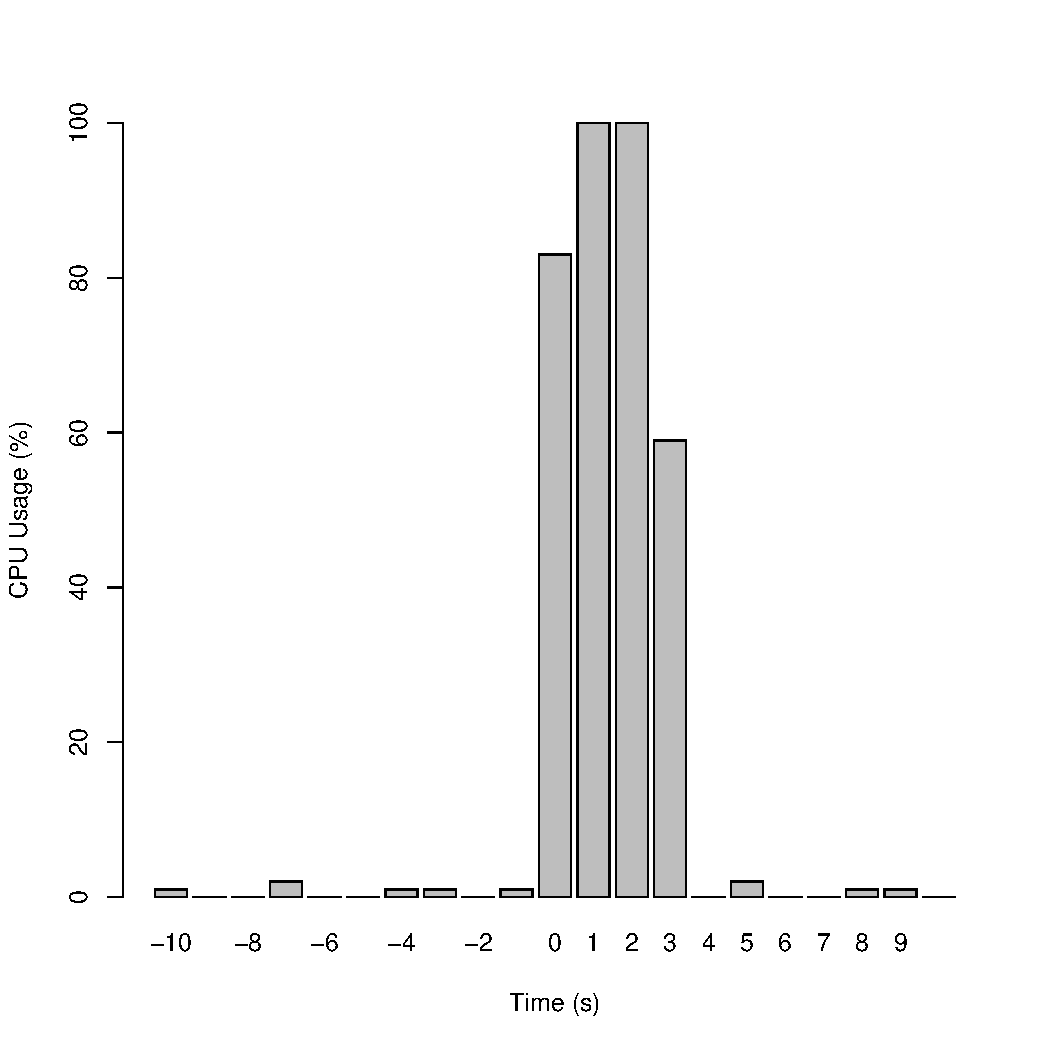
\includegraphics[width=0.6\hsize]{experiment_data_128_0001_mmeperf.pdf}
%   \caption{$t=0$で128台のUEがアタッチ処理を実行した時のCPU負荷(実験データそのまま)}
%   \label{experiment_data_128_0001_mmeperf}
% \end{figure}
% \begin{figure}[htbp]
%   \centering
%   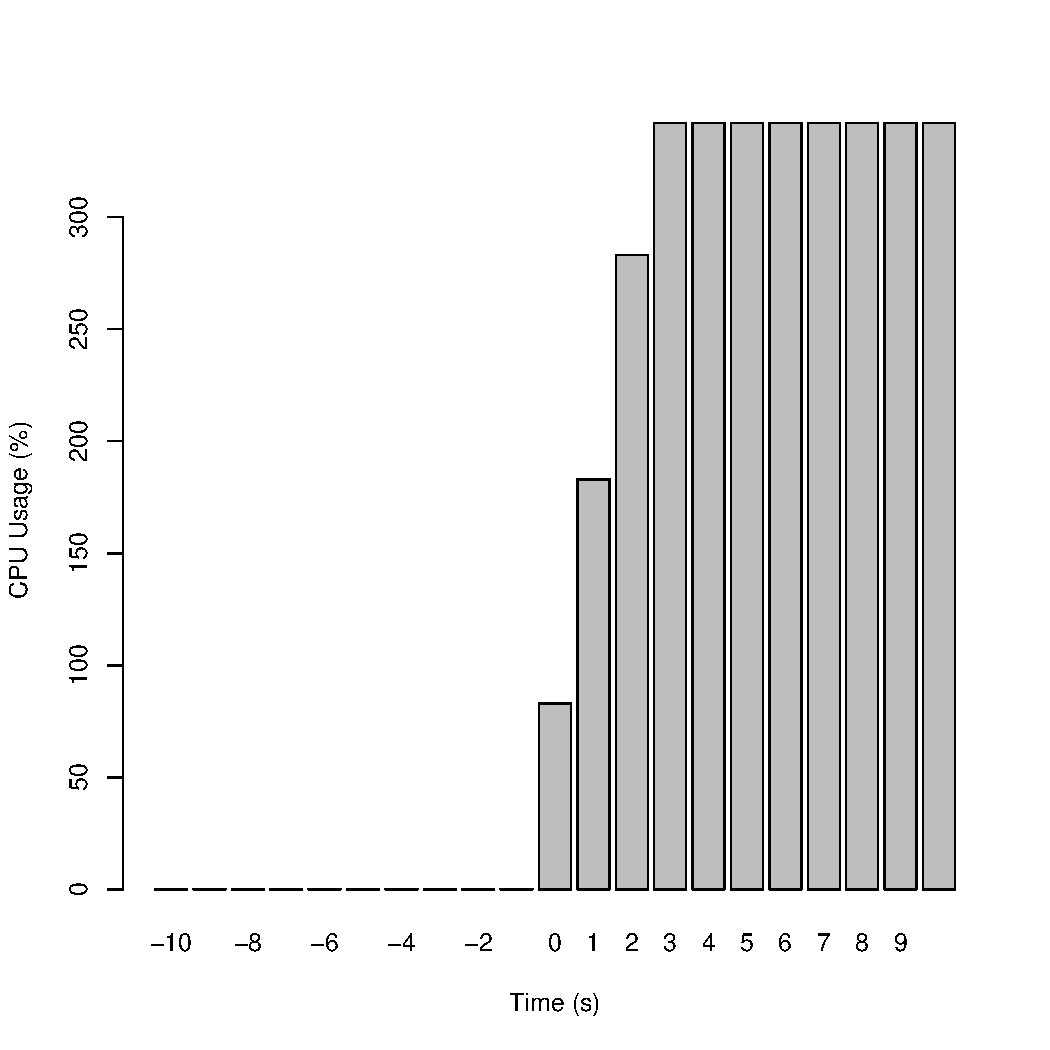
\includegraphics[width=0.6\hsize]{experiment_data_128_0001_mmeperf_estimate.pdf}
%   \caption{$t\geq0$で毎秒128台のUEがアタッチ処理を実行した時のCPU負荷(推定)}
%   \label{experiment_data_128_0001_mmeperf_estimate}
% \end{figure}
%
% \begin{figure}[htbp]
%   \centering
%   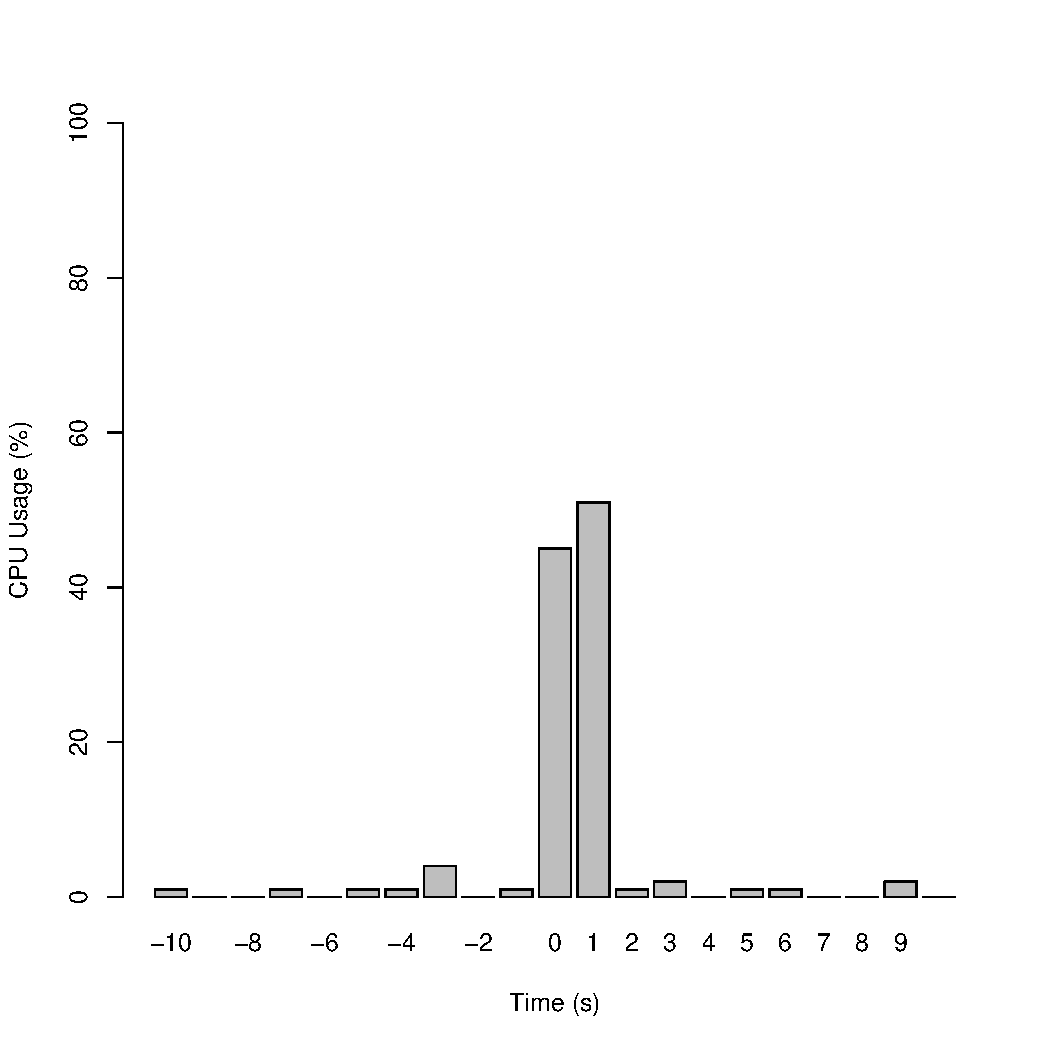
\includegraphics[width=0.6\hsize]{experiment_data_64_0001_mmeperf.pdf}
%   \caption{$t=0$で64台のUEがアタッチ処理を実行した時のCPU負荷(実験データそのまま)}
%   \label{experiment_data_64_0001_mmeperf}
% \end{figure}
% \begin{figure}[htbp]
%   \centering
%   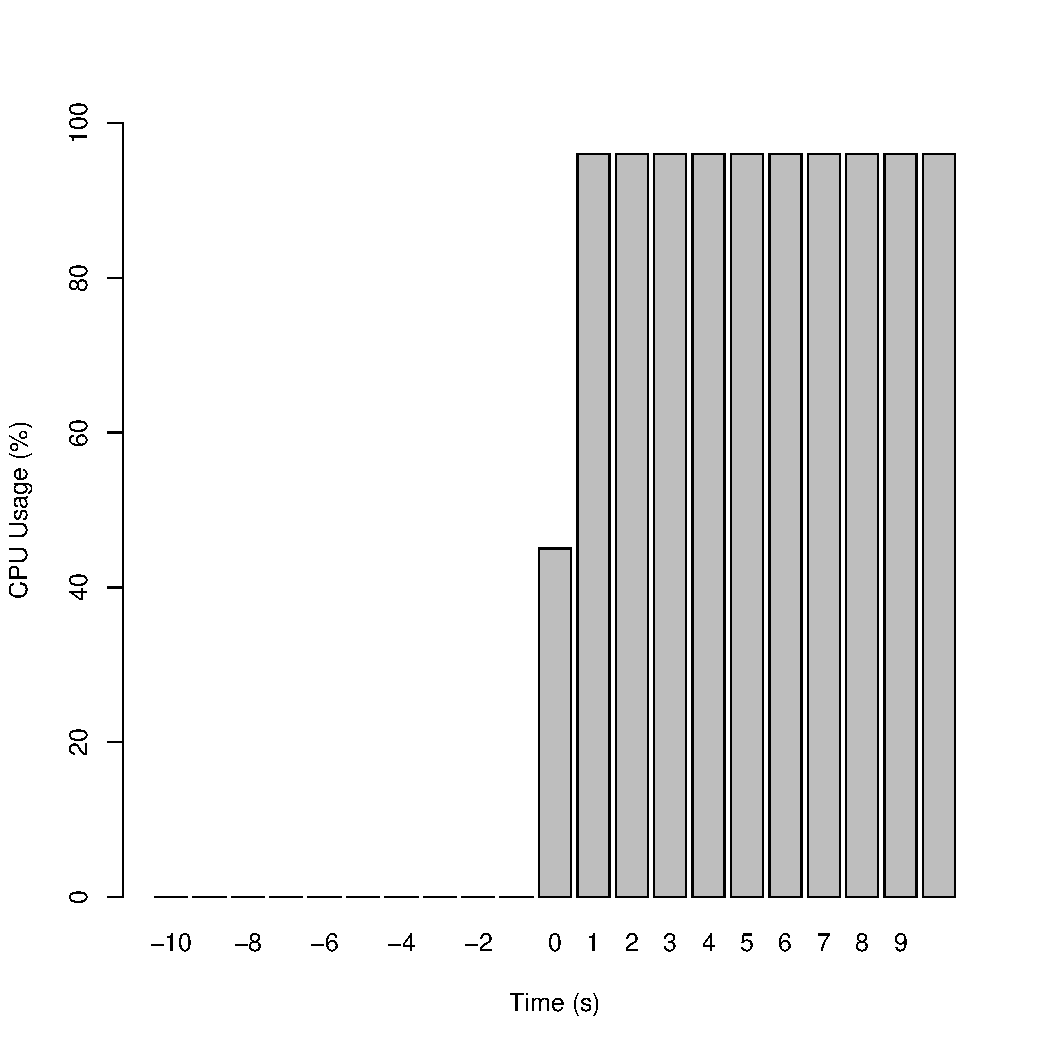
\includegraphics[width=0.6\hsize]{experiment_data_64_0001_mmeperf_estimate.pdf}
%   \caption{$t\geq0$で毎秒64台のUEがアタッチ処理を実行した時のCPU負荷(推定)}
%   \label{experiment_data_64_0001_mmeperf_estimate}
% \end{figure}
%
% \begin{figure}[htbp]
%   \centering
%   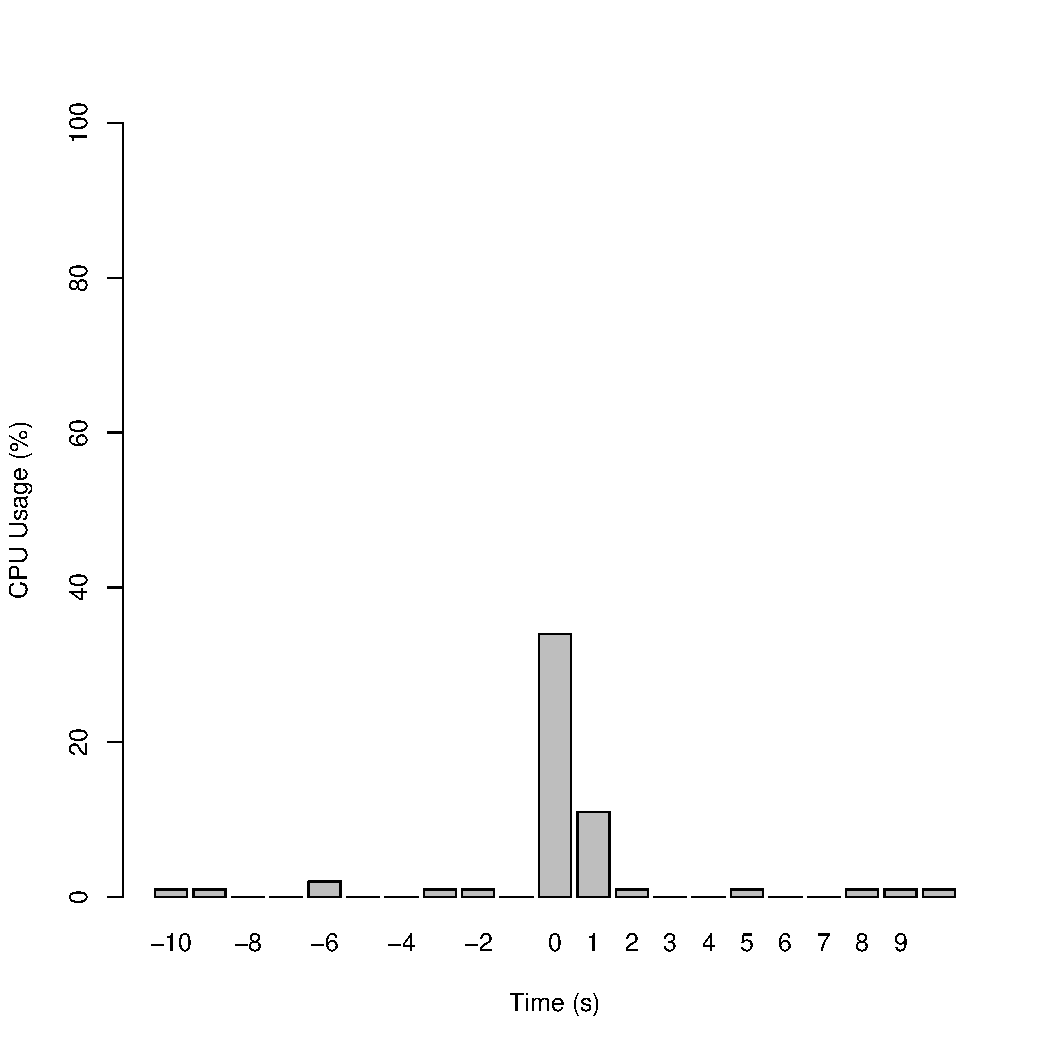
\includegraphics[width=0.6\hsize]{experiment_data_32_0001_mmeperf.pdf}
%   \caption{$t=0$で32台のUEがアタッチ処理を実行した時のCPU負荷(実験データそのまま)}
%   \label{experiment_data_32_0001_mmeperf}
% \end{figure}
% \begin{figure}[htbp]
%   \centering
%   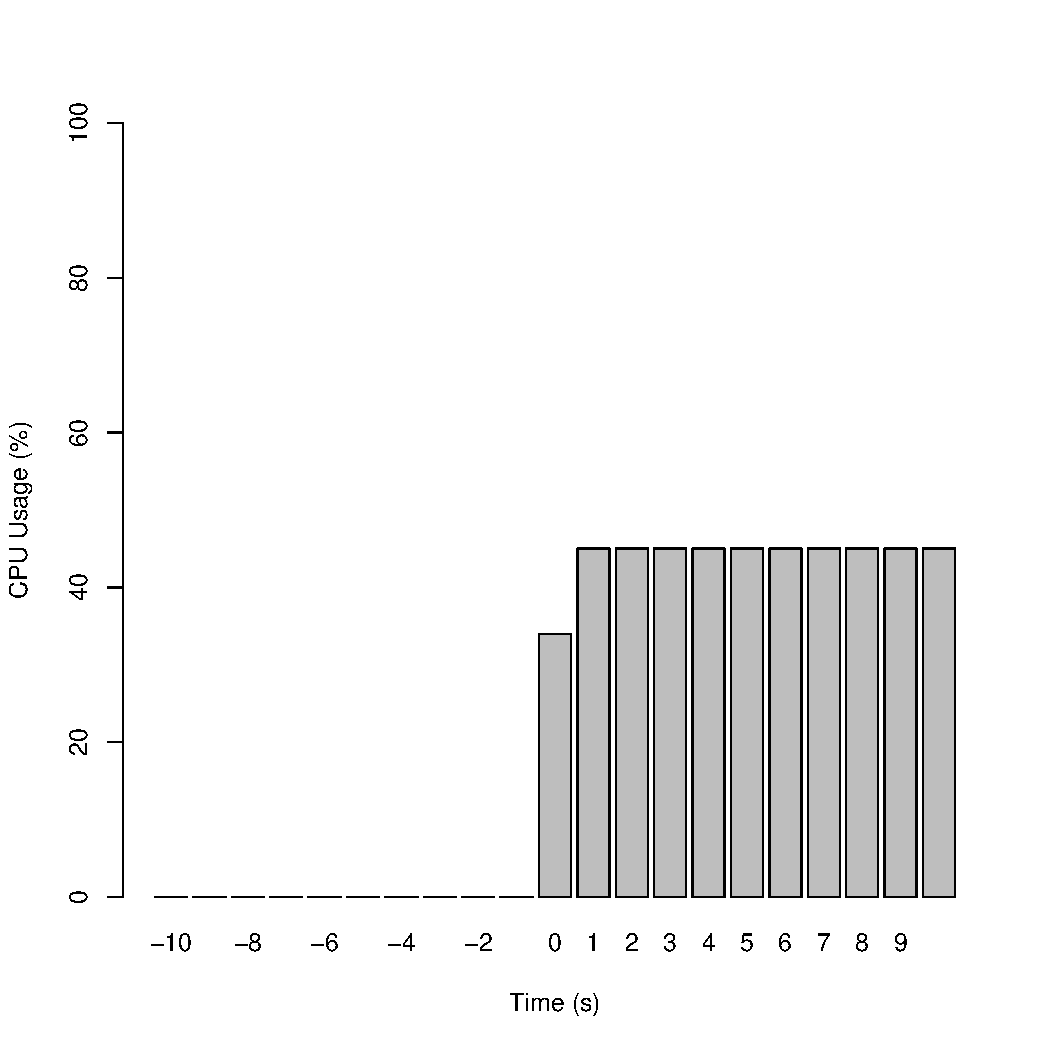
\includegraphics[width=0.6\hsize]{experiment_data_32_0001_mmeperf_estimate.pdf}
%   \caption{$t\geq0$で毎秒32台のUEがアタッチ処理を実行した時のCPU負荷(推定)}
%   \label{experiment_data_32_0001_mmeperf_estimate}
% \end{figure}


以上の調査から、毎秒約80台のUEがアタッチ処理を実行する際に発生するシグナリング負荷以下ならば、MMEは処理可能であると言える。
図\ref{signaling}に示すように、MMEは1つのアタッチ処理完了するために、15回のシグナリング処理を行っている。
このことから、毎秒約1200回のシグナリング負荷以下であれば、CPUは過負荷にならないと推定できる。
\begin{figure}[htbp]
  \centering
  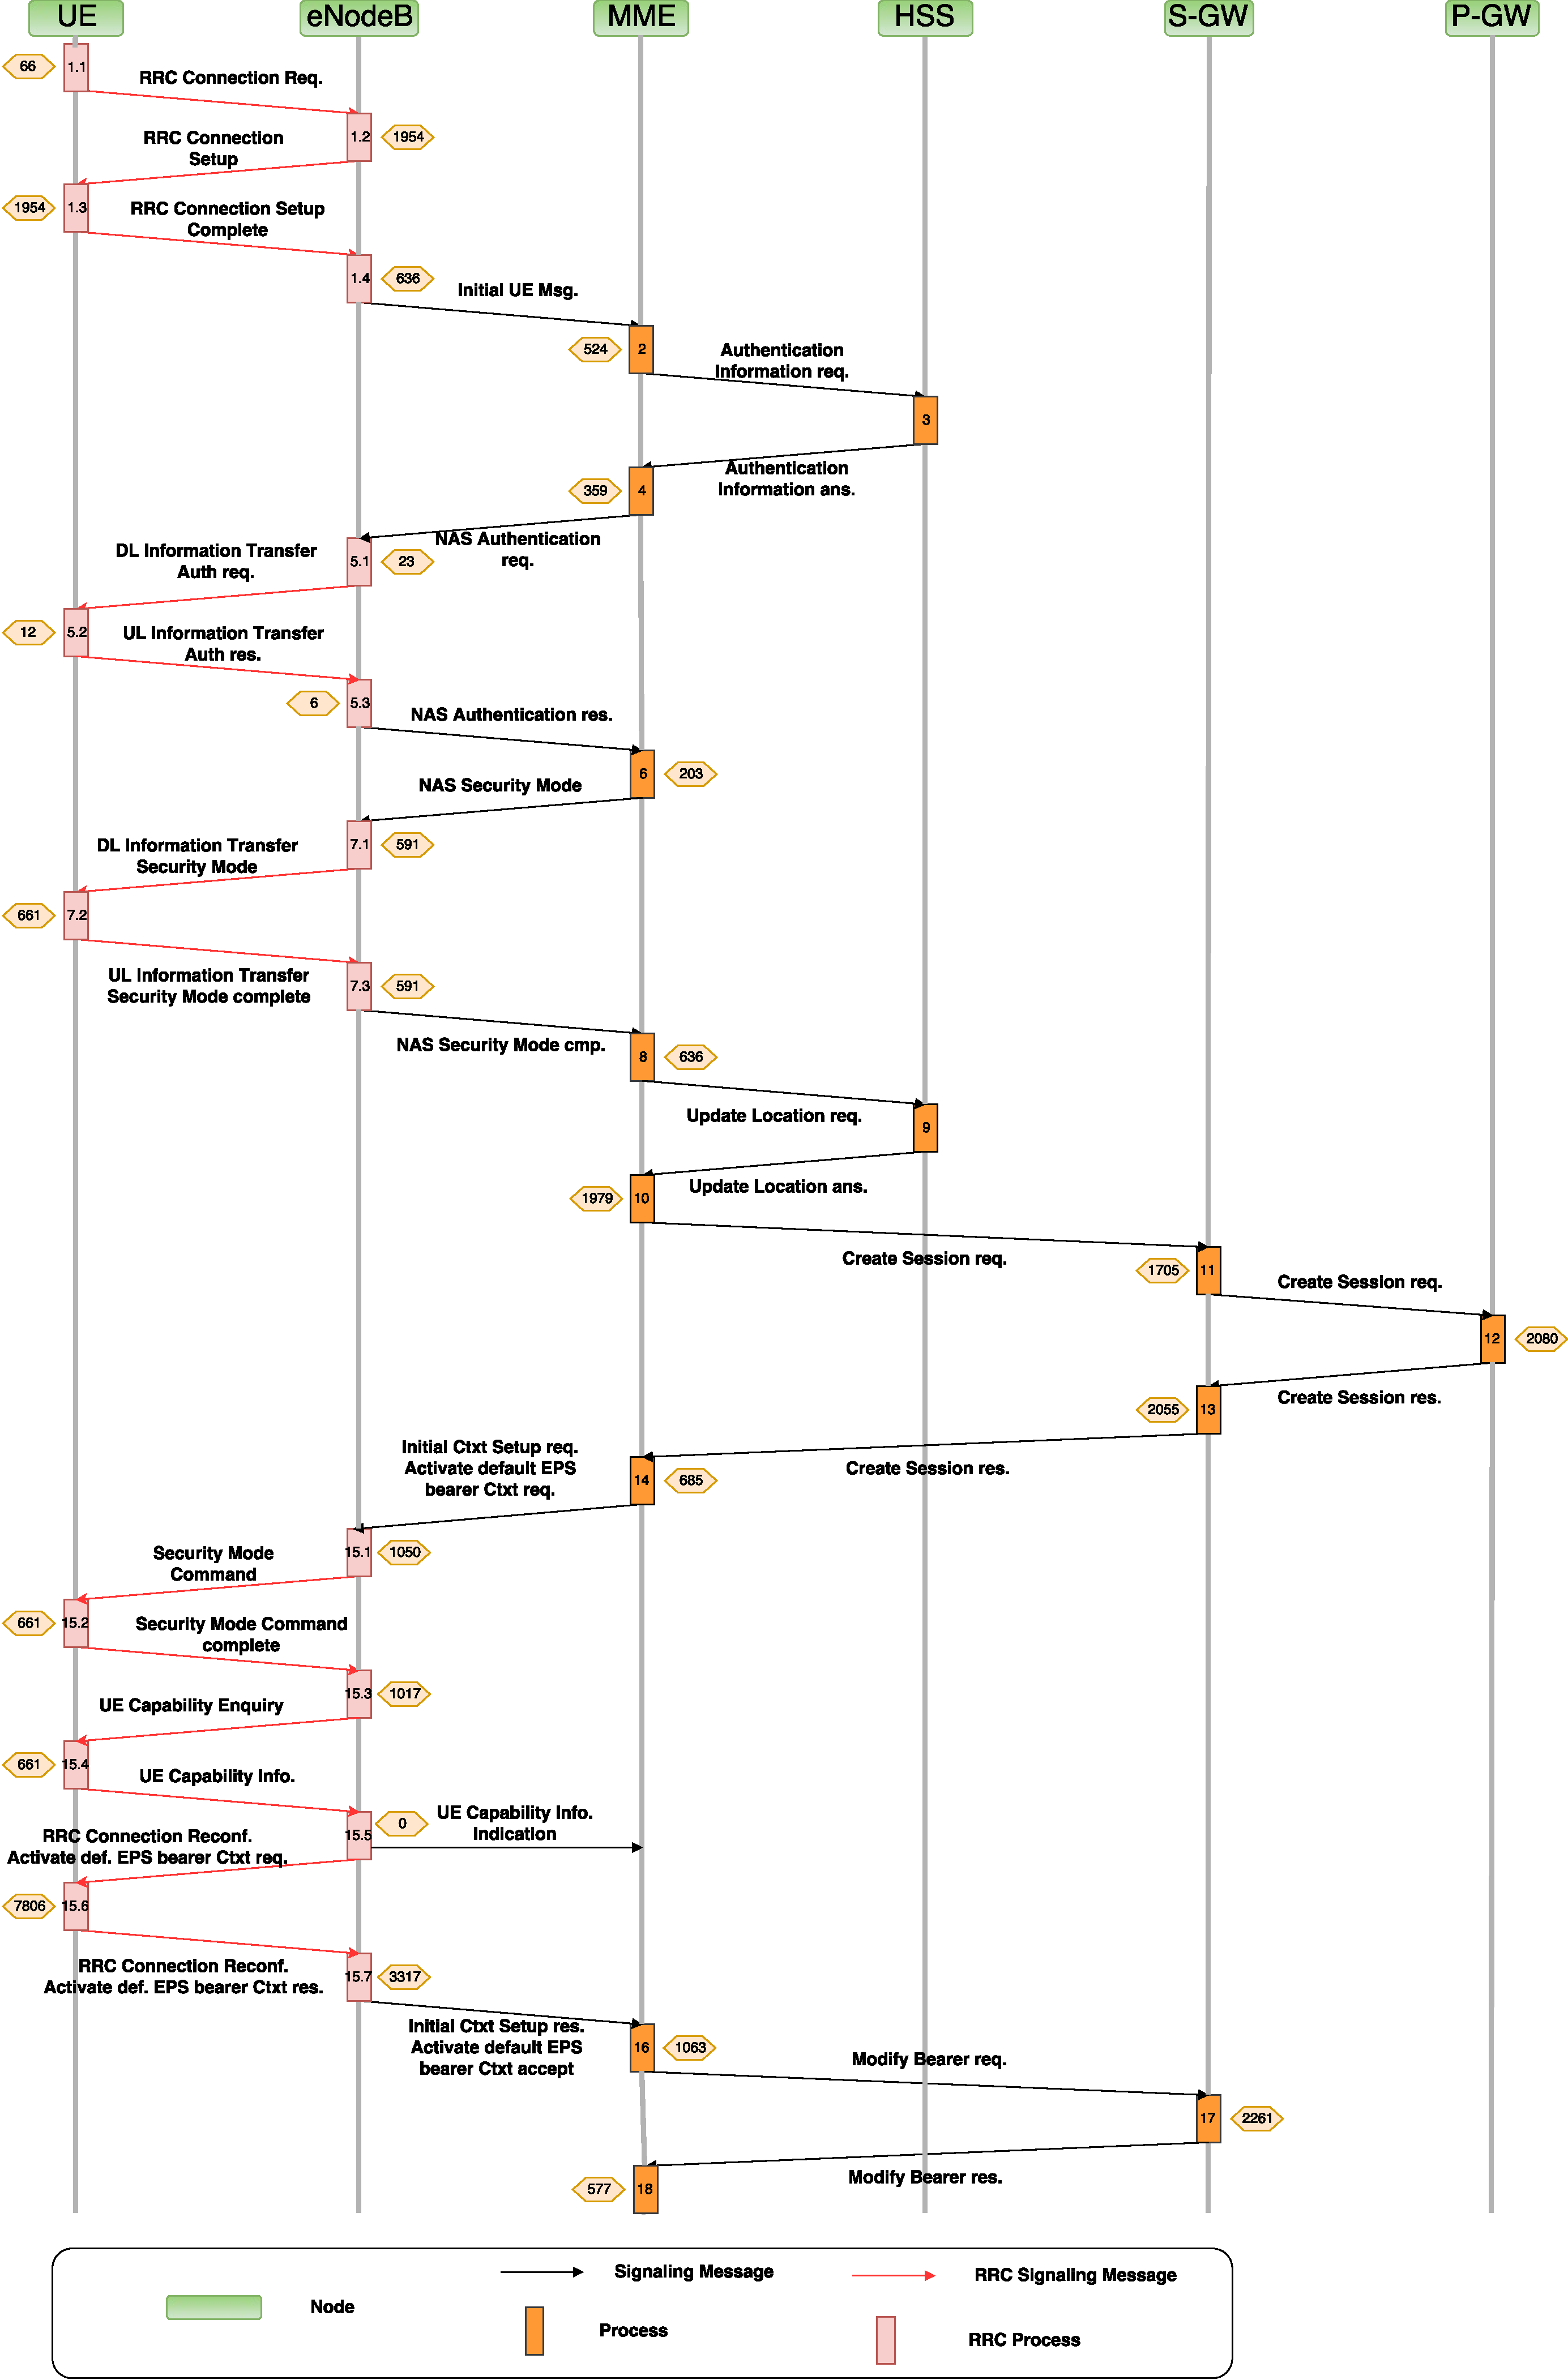
\includegraphics[width=0.9\hsize]{signaling.pdf}
  \caption{}
  \label{signaling}
\end{figure}

\clearpage
  \section{今後の予定}
  \begin{itemize}
    \item UEの通信周期の分布やデータサイズなど、様々なパラメータを変化させた場合の試算を行う。
    \item MME負荷の試算
    \item 必要に応じてSGWやeNodeBなどのメモリ負荷も調査する。
    \item Connected Inactive状態において``状態遷移を伴わないデータ送信"が可能なデータ量を調査する。
  \end{itemize}

\section*{\addcontentsline{toc}{section}{参考文献}}
\bibliographystyle{IEEEtran}
\bibliography{/Users/t-adachi/Documents/study/Bibliography/bib/hpt_core_network/myBib/LABbiblio,/Users/t-adachi/Documents/study/Bibliography/bib/hpt_core_network/Study_Group_Bibtex/bib/hptCoreNetwork_Study}
\end{document}
